% Also note that the "draftcls" or "draftclsnofoot", not "draft", option
% should be used if it is desired that the figures are to be displayed in
% draft mode.
\documentclass[10pt,journal,letterpaper,compsoc]{IEEEtran}
%\documentclass[10pt,journal,letterpaper,compsoc,draftcls]{IEEEtran}
%\documentclass[10pt,journal,letterpaper,compsoc,draft]{IEEEtran}

%% NOTE: THIS PACKAGE LOOKS AWESOME FOR TODOS:
%% http://www.tex.ac.uk/ctan/macros/latex/contrib/todonotes/todonotes.pdf

\usepackage{graphicx}
\usepackage{amsmath}
\usepackage{booktabs}
\usepackage{multirow}
\usepackage{todonotes}

\usepackage{pgf,tikz}
\usepackage{color,xcolor}
\usepackage{amsmath,amssymb}
\usepackage{rotating}
\newcommand{\drawFluent}[3]{
\draw [thick,cyan,fill=cyan!50] (#1,#2+#3) -- (#1-#3*0.866,#2-#3*0.5) -- (#1+#3*0.866,#2-#3*0.5) -- cycle;
}
\newcommand{\drawHollowFluent}[3]{
\draw [thick,cyan,fill=white] (#1,#2+#3) -- (#1-#3*0.866,#2-#3*0.5) -- (#1+#3*0.866,#2-#3*0.5) -- cycle;
}
\newcommand{\drawHiddenFluent}[3]{
\draw [very thick,dotted,cyan] (#1,#2+#3) -- (#1-#3*0.866,#2-#3*0.5);
\draw [very thick,dotted,cyan] (#1-#3*0.866,#2-#3*0.5) -- (#1+#3*0.866,#2-#3*0.5);
\draw [very thick,dotted,cyan] (#1+#3*0.866,#2-#3*0.5) -- (#1,#2+#3);
}
\newcommand{\drawHiddenFluentST}[3]{
\draw [very thick,dotted,red] (#1,#2+#3) -- (#1-#3*0.866,#2-#3*0.5);
\draw [very thick,dotted,red] (#1-#3*0.866,#2-#3*0.5) -- (#1+#3*0.866,#2-#3*0.5);
\draw [very thick,dotted,red] (#1+#3*0.866,#2-#3*0.5) -- (#1,#2+#3);
}
\newcommand{\drawAction}[3]{
\draw [thick,gray,fill=lime] (#1,#2+#3) -- (#1-#3,#2) -- (#1,#2-#3) -- (#1+#3,#2) -- cycle;
}
\newcommand{\drawInertialAction}[3]{
\draw [thick,gray,fill=lime] (#1,#2+#3) -- (#1-#3,#2) -- (#1,#2-#3) -- (#1+#3,#2) -- cycle;
\draw [very thick,red] (#1,#2) circle (#3*0.5);
\draw [very thick,red] (#1-#3*0.5*0.707,#2+#3*0.5*0.707) -- (#1+#3*0.5*0.707,#2-#3*0.5*0.707);
}
\newcommand{\drawInferredValue}[3]{
\draw [very thick,dotted,cyan] (#1-#3,#2) -- (#1+#3,#2);
}
\newcommand{\drawCausalLink}[3]{
\draw [very thick,red,->] (#1-#3,#2) -- (#1+#3,#2);
}
\newcommand{\drawTrigger}[3]{
\draw [thick,blue,->] (#1-#3,#2) -- (#1+#3,#2);
}
\newcommand{\drawTransitPP}[3]{
\draw [thick,fill=white] (#1,#2) circle (#3);
\draw [thick] (#1-#3*0.5,#2+#3*0.5) -- (#1+#3*0.5,#2+#3*0.5);
}
\newcommand{\drawTransitNN}[3]{
\draw [thick,fill=white] (#1,#2) circle (#3);
\draw [thick] (#1-#3*0.5,#2-#3*0.5) -- (#1+#3*0.5,#2-#3*0.5);
}
\newcommand{\drawTransitPN}[3]{
\draw [thick,fill=white] (#1,#2) circle (#3);
\draw [thick] (#1-#3*0.5,#2+#3*0.5) -- (#1,#2+#3*0.5) -- (#1,#2-#3*0.5) -- (#1+#3*0.5,#2-#3*0.5);
}
\newcommand{\drawTransitNP}[3]{
\draw [thick,fill=white] (#1,#2) circle (#3);
\draw [thick] (#1-#3*0.5,#2-#3*0.5) -- (#1,#2-#3*0.5) -- (#1,#2+#3*0.5) -- (#1+#3*0.5,#2+#3*0.5);
}

%%%%%%%%%%%%%%%%%%%%% TODOS %%%%%%%%%%%%%%%%%%%%
%%% TODO: double check my notation!
% \mathcal{E} for energy
% E for expectation
% \textrm{C}, \textrm{T}, \textrm{S} for temporal, causal, spatial

%%% TODO: screen saver or screensaver (note: use no space)

%%% TODO: use \textrm{ST}, not \mathrm{ST}

%%% TOOD: clean up notation mess with pg_t(a,b)

%%%%%%%%%%%%%%%%%%%%%%%%%%%%%%%%%%%%%%%%%%%%%%%




\usepackage[ruled,lined]{algorithm2e}
% *** SPECIALIZED LIST PACKAGES ***
%
%\usepackage{algorithmic}
% algorithmic.sty was written by Peter Williams and Rogerio Brito.
% This package provides an algorithmic environment fo describing algorithms.
% You can use the algorithmic environment in-text or within a figure
% environment to provide for a floating algorithm. Do NOT use the algorithm
% floating environment provided by algorithm.sty (by the same authors) or
% algorithm2e.sty (by Christophe Fiorio) as IEEE does not use dedicated
% algorithm float types and packages that provide these will not provide
% correct IEEE style captions. The latest version and documentation of
% algorithmic.sty can be obtained at:
% http://www.ctan.org/tex-archive/macros/latex/contrib/algorithms/
% There is also a support site at:
% http://algorithms.berlios.de/index.html
% Also of interest may be the (relatively newer and more customizable)
% algorithmicx.sty package by Szasz Janos:
% http://www.ctan.org/tex-archive/macros/latex/contrib/algorithmicx/



% correct bad hyphenation here
\hyphenation{op-tical net-works semi-conduc-tor}


\begin{document}

\title{Inferring Hidden Status and Intents \\ in Video by Causal Reasoning% and Actions:\\Joint Inference through Causality
}
%


\author{Amy~Fire
        and~Song-Chun~Zhu%,~\IEEEmembership{Fellow,~IEEE}% <-this % stops a space
\IEEEcompsocitemizethanks{\IEEEcompsocthanksitem The authors are with the Department of Statistics, University of California, Los Angeles, CA 90095.\protect\\
% note need leading \protect in front of \\ to get a newline within \thanks as
% \\ is fragile and will error, could use \hfil\break instead.
E-mail: amy.fire@ucla.edu, sczhu@stat.ucla.edu}% <-this % stops a space
\thanks{}}




% The paper headers
\markboth{FOR REVIEW: TPAMI}%
{Fire and Zhu: Inferring Hidden Fluents Using Action and Causality}
% The only time the second header will appear is for the odd numbered pages
% after the title page when using the twoside option.
% 
% *** Note that you probably will NOT want to include the author's ***
% *** name in the headers of peer review papers.                   ***
% You can use \ifCLASSOPTIONpeerreview for conditional compilation here if
% you desire.





% for Computer Society papers, we must declare the abstract and index terms
% PRIOR to the title within the \IEEEcompsoctitleabstractindextext IEEEtran
% command as these need to go into the title area created by \maketitle.
\IEEEcompsoctitleabstractindextext{%

\begin{abstract}
%\boldmath
This paper presents a method to infer the hidden statuses of objects or intents of agents (these are called fluents) from video through causal reasoning. Event analysis from video provides detections of status changes (light turn on, turn off) and possible actions, given a number of objects in the scene that we care about (ex: cup, etc).  These probabilistic detections, however, may be incorrect or ambiguous.  Over time, we use dynamic programming to isolate the best interpretation of the scene, jointly considering detections and causal knowledge.  Transition probabilities are dictated by 2 things: 1) the survival analysis histogram (given certain time t duration, how likely the status change during this time duration).  2) if observe a certain action, then how likely change from A to B.  if don't observe anything, then this is inertial probability (how things to work).  Our modifications to the dynamic programming algorithm accomodate the non-linearity by allowing the insertion of a new action or fluent change.  

Our system outputs the hidden status that is not observable in the video, through causal inference.  The model incorporates causal reasoning with spatio-temporal detection to generate multiple interpretations of what is transpiring in a scene and to rank those interpretations according to probability.  We show that such interpretations can be used to correct (mis)detections of fluents and events in video; results are comparable to humans' performance in reasoning values of hidden fluents.
\end{abstract}

% Note that keywords are not normally used for peer review papers.
\begin{keywords}
Causal inference, commonsense reasoning, event analysis, fluents
\end{keywords}}


% make the title area
\maketitle


\IEEEdisplaynotcompsoctitleabstractindextext


\IEEEpeerreviewmaketitle

\section{Introduction}


\todo[inline]{RESTRUCTURE INTRODUCTION}.  

\todo[inline]{--- PARAGRAPH 1 -- general statement about teleological stance and causal effects}

Motivation: World/Environment we live in has been designed in a way to reflect cause and effect relationships.  Any action is planned to achieve a change in the world: either as a status of object, or the hidden mind.  

So we take the teleological stance.  action is taken, triggered by certain condition/status of object.  at the same time, they are aimed to change the status (of object or the agents mind) of the world.  For example, the elevator: push the elevator button, it lights up...  Our world was designed in such a way...  By dialog too... 

Almost every action/event has a goal to change the world.  And every action was triggered by condition.  However, many of this conditions (object state or fluent/state of the mind) are hidden.  So only a portion are observable.  


\todo[inline]{--- PARAGRAPH 2 -- show some examples -- scenario}

Focus on examples of drinking (water lower whether cup empty or not) and locked door and approaching car (intent: maybe forgot key).


\todo[inline]{--- PARAGRAPH 3 -- explicit/concrete}
make explicit: In those examples, fluent triggers action.  thirsty triggers getting cup.  action triggers fluent change: after drinking water, the cup was empty.  get water: becomes full.

and this process includes inference and forward/backward in time....


\todo[inline]{--- PARAGRAPH 4 --}
say what is input/output again.  In this paper,...




[[FROM NIPS REVIEWS: The general question addressed in the paper is incredibly important (and challenging). The applications of this approach are wide reaching not only for applied questions (automatic recognition of the content of video sequences) but also for theoretical understanding of how humans resolve similar uncertainty in their daily reasoning. The authors nicely position this work along side not only state-of-the-art machine vision systems but also core issues in cognitive science. ]]


\IEEEPARstart{H}{umans} are capable of employing commonsense reasoning to extend inference beyond observation.  For example, consider the following office scene:  
\begin{enumerate}
\item A person sitting behind a computer screen reaches over and moves the mouse, then starts typing.  What is the monitor's display status?  Is the computer on? Asleep?  
\item Later, the person grabs a cup and moves to the water dispenser. Why did he get water?  Was he thirsty?  Is the cup empty?  
\item The agent moves to the wall and raises his arm.  The light goes out.  Did the agent turn the light off?
\end{enumerate}

The values of the fluents in the first two scenes (i.e., the statuses of the objects, such as whether the monitor display is active and whether the man is thirsty) are hidden, but an intelligent observer equipped with commonsense causality can answer the posed questions by connecting information.  Figure~\ref{fig:largepg} represents one possible inference process in which values of hidden fluents are filled in as preconditions or effects of the observed actions.  Even without seeing the screen or the computer, an observer can infer that the agent in the scene moved the mouse to wake the monitor, and that when the typing begins, both the computer and the monitor are likely on.  In the second scene, an observer can infer that the agent's actions were triggered by his thirst and the emptiness of the cup.  

\missingfigure{[[MOVE FIGURE 1 EXPLANATION TO SECTION 1.3 (JOINT INFERENCE)]]}

Finally, in the third scene, the fluent value is observable, but the precise action is harder to detect.  Without seeing the agent ``flipping the light switch'', the observer can still reason the agent performed the action based on the observed effects.

\begin{figure*}[hbtp]
\centering
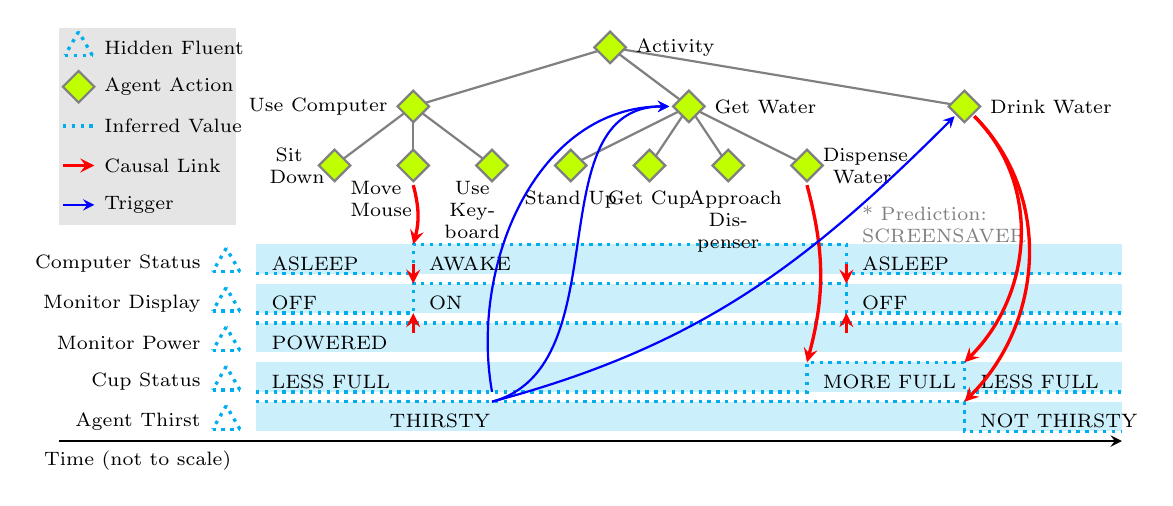
\begin{tikzpicture}[scale=0.5,>=stealth]
\scriptsize
\draw [thick,->] (-3,0) -- (24,0);\node at (-1,-0.5) {Time (not to scale)};
\fill [cyan!20] (2,0.25) rectangle (24,1);\draw [very thick,dotted,cyan] (2,1) -- (20,1) -- (20,0.25) -- (24,0.25);
\fill [cyan!20] (2,1.25) rectangle (24,2);\draw [very thick,dotted,cyan] (2,1.25) -- (16,1.25) -- (16,2) -- (20,2) -- (20,1.25) -- (24,1.25);
\fill [cyan!20] (2,2.25) rectangle (24,3);\draw [very thick,dotted,cyan] (2,3) -- (24,3);
\fill [cyan!20] (2,3.25) rectangle (24,4);\draw [very thick,dotted,cyan] (2,3.25) -- (6,3.25) -- (6,4) -- (17,4) -- (17,3.25) -- (24,3.25);
\fill [cyan!20] (2,4.25) rectangle (24,5);\draw [very thick,dotted,cyan] (2,4.25) -- (6,4.25) -- (6,5) -- (17,5) -- (17,4.25) -- (24,4.25);
\drawHiddenFluent{1.25}{0.5}{0.4};\node at (1,0.5) [label=left:Agent Thirst] {};
\drawHiddenFluent{1.25}{1.5}{0.4};\node at (1,1.5) [label=left:Cup Status] {};
\drawHiddenFluent{1.25}{2.5}{0.4};\node at (1,2.5) [label=left:Monitor Power] {};
\drawHiddenFluent{1.25}{3.5}{0.4};\node at (1,3.5) [label=left:Monitor Display] {};
\drawHiddenFluent{1.25}{4.5}{0.4};\node at (1,4.5) [label=left:Computer Status] {};
\fill [gray!20] (-3,5.5) rectangle (1.5,10.5);
\drawHiddenFluent{-2.5}{10}{0.4};\node at (-2.25,10) [label=right:Hidden Fluent] {};
\drawAction{-2.5}{9}{0.4};\node at (-2.25,9) [label=right:Agent Action] {};
\drawInferredValue{-2.5}{8}{0.4};\node at (-2.25,8) [label=right:Inferred Value] {};
\drawCausalLink{-2.5}{7}{0.4};\node at (-2.25,7) [label=right:Causal Link] {};
\drawTrigger{-2.5}{6}{0.4};\node at (-2.25,6) [label=right:Trigger] {};
%
\draw [thick,gray] (11,10) -- (6,8.5);
\draw [thick,gray] (11,10) -- (13,8.5);
\draw [thick,gray] (11,10) -- (20,8.5);
\draw [thick,gray] (6,8.5) -- (4,7);
\draw [thick,gray] (6,8.5) -- (6,7);
\draw [thick,gray] (6,8.5) -- (8,7);
\draw [thick,gray] (13,8.5) -- (10,7);
\draw [thick,gray] (13,8.5) -- (12,7);
\draw [thick,gray] (13,8.5) -- (14,7);
\draw [thick,gray] (13,8.5) -- (16,7);
\drawAction{11}{10}{0.4};\node at (11.25,10) [label=right:Activity] {};
\drawAction{6}{8.5}{0.4};\node at (5.75,8.5) [label=left:Use Computer] {};
\drawAction{13}{8.5}{0.4};\node at (13.25,8.5) [label=right:Get Water] {};
\drawAction{20}{8.5}{0.4};\node at (20.25,8.5) [label=right:Drink Water] {};
\drawAction{4}{7}{0.4};\node at (3.75,7) [label=left:\parbox{.5cm}{\centering Sit Down}] {};
\drawAction{6}{7}{0.4};\node at (5,7) [label=below:\parbox{.6cm}{\centering Move Mouse}] {};
\drawAction{8}{7}{0.4};\node at (7.5,7) [label=below:\parbox{1cm}{\centering Use Keyboard}] {};
\drawAction{10}{7}{0.4};\node at (10,6.75) [label=below:Stand Up] {};
\drawAction{12}{7}{0.4};\node at (12,6.75) [label=below:Get Cup] {};
\drawAction{14}{7}{0.4};\node at (14,6.75) [label=below:\parbox{1cm}{\centering Approach Dispenser}] {};
\drawAction{16}{7}{0.4};\node at (16,7) [label=right:\parbox{1cm}{\centering Dispense Water}] {};
%
\node at (17,5.5) [label=right:\parbox{2cm}{\color{gray}* Prediction:\\SCREENSAVER}] {};
\node at (2,4.5) [label=right:ASLEEP] {};
\node at (6,4.5) [label=right:AWAKE] {};
\node at (17,4.5) [label=right:ASLEEP] {};
\node at (2,3.5) [label=right:OFF] {};
\node at (6,3.5) [label=right:ON] {};
\node at (17,3.5) [label=right:OFF] {};
\node at (2,2.5) [label=right:POWERED] {};
\node at (2,1.5) [label=right:LESS FULL] {};
\node at (16,1.5) [label=right:MORE FULL] {};
\node at (20,1.5) [label=right:LESS FULL] {};
\node at (5,0.5) [label=right:THIRSTY] {};
\node at (20,0.5) [label=right:NOT THIRSTY] {};
%
\draw [very thick,red,->] (6,6.5) [out=-75,in=75] to (6,5);
\draw [very thick,red,->] (6,4.5) -- (6,4);
\draw [very thick,red,->] (6,2.75) -- (6,3.25);
\draw [very thick,red,->] (16,6.5) [out=-75,in=75] to (16,2);
\draw [very thick,red,->] (17,4.5) -- (17,4);
\draw [very thick,red,->] (17,2.75) -- (17,3.25);
\draw [very thick,red,->] (20.25,8.25) [out=-45,in=45] to (20,2);
\draw [very thick,red,->] (20.25,8.25) [out=-45,in=45] to (20,1);
%
\draw [thick,blue,->] (8,1.25) [out=100,in=180] to (12.5,8.5);
\draw [thick,blue,->] (8,1) [out=15,in=180] to (12.5,8.5);
\draw [thick,blue,->] (8,1) [out=15,in=-135] to (19.75,8.25);
\end{tikzpicture}
%\includegraphics[trim = .25in 1.25in .7in 2.25in, clip, width=.95\linewidth]{largepg.pdf}
\caption{Illustration of the scenarios from the beginning. Observed actions are used to infer values of hidden fluents, and values of observed fluents are similarly used to infer hidden actions.  The inference process extends beyond single instances, providing coherent reasoning solutions both backward and forward in time. 
TODO: fix word spacing, make fill page width, add turning off light.
\label{fig:largepg}}
\end{figure*}

\todo[inline]{FIGURE 1: DITCH HIERARCHY (keep only actions at top).   (OBSERVED OR INFERRED).  AND FLUENT CHANGE DETECTION--OBSERVABLE FLUENT CHANGE FOR THE SEQUENCE.  STILL HAVE TRIGGERS AND CAUSAL EFFECTS.  GET RID OF T-AOG.}

Inferring fluents of objects and agents together with agent's actions is crucial to understanding that agent's actions, intents, and probable future actions.  Therefore, the ability to jointly infer the values of hidden fluents with actions is an important step for artificial-intelligence applications such as constructing situationally aware robots and developing intelligent video-surveillance systems.  These reasoning and inference tasks, however, have not been studied in current vision literature. This paper presents methods for jointly inferring values of fluents with agent actions from video input.



\subsection{Fluents of objects and fluents of the mind}
%1.1: WHAT IS FLUENTS

First introduced by Newton \cite{Newton}, the concept of fluents has been adapted in the commonsense reasoning literature to describe time-varying statuses of objects \cite{CommonsenseReasoning}.  Although both describe objects, ``fluents'' are defined quite differently from ``attributes'', which have received much attention in recent vision literature (e.g., \cite{lampert2009learning}).  Whereas the values of attributes such as the color or texture of an object remain constant over the course of a video, the values of fluents change.   The research described in this paper examines two kinds of fluents: 
\begin{enumerate}
\item Object fluents, e.g., whether a monitor is powered, a light is on, a cup has water, or a door is locked.   Because of limitations on visibility and detectability, the values of these fluents are often hidden.  They are connected to actions as preconditions or effects.  
%TODO NEXT TIME: Door locked.
%Object fluents, e.g. whether the power to a monitor is on or not,
%   Whether a cup has water, or whether a door is locked.  These fluents are
%   mostly invisible, let alone detecting them in images, but they are 
%   tied to human actions as preconditions and causal effects
%    (remove the repeated words on line 053)
%   and thus play important roles in event understanding
\item Fluents of the mind, e.g., whether an agent is thirsty, hungry, or tired.  An agent's state of mind is completely hidden.  Fluents of the mind act as triggers to an agent's actions.
\end{enumerate}


\subsection{Fluents over time}


[[moved here to FINISH explanation of all fluents (HAD DONE FLUENTS OF OBJECTS, THEN FLUENTS OF MIND, NOW FLUENTS OVER TIME]]

Whereas the work in \cite{morrow2012pami} seeks only a causal explanation at $t$, it does not consider how the values at each time are connected.  

As time increments, $t = 1, 2, \ldots, n$, the fluent $F$ takes on a sequence of values, $F(t) = f_t$, or $(f_1, f_2, \ldots, f_n)$.  The values in the sequence, however, are not independent from each other---at least two dependencies exist.  

First, the fluent value at $t-1$, together with actions in recent history, restrict the values available for the fluent at $t$.  For example, if the light is on at $t$ and someone touches the light switch, then it is {\em not} possible that touching the switch changed the light from off to on.  This obvious statement forms an important consistency constraint on the sequence.  In particular, this constraint allows the model presented in this paper to overcome imperfect spatio-temporal detections from video, providing a coherent sequence of values for the fluent over the course of the video.

The second dependency originates due to the duration a fluent has maintained a particular value without agent intervention.  Where some changes in fluent values are attributable to causing actions, other changes occur due to a strong dependence on time.  The duration a fluent has maintained a particular value provides information for when a transition to another state will occur.  The screensaver on the computer, for example, changes after a pre-specified allotment of time, and this amount of time is usually in 5 minute increments.  Agents also experience duration constraints, where, for example, the longer a person goes without drinking, the sooner he will be thirsty.  

\todo[inline]{inlude uniform histogram for fluents that don't have timer mechanism.}

\begin{figure}[htp]
\centering
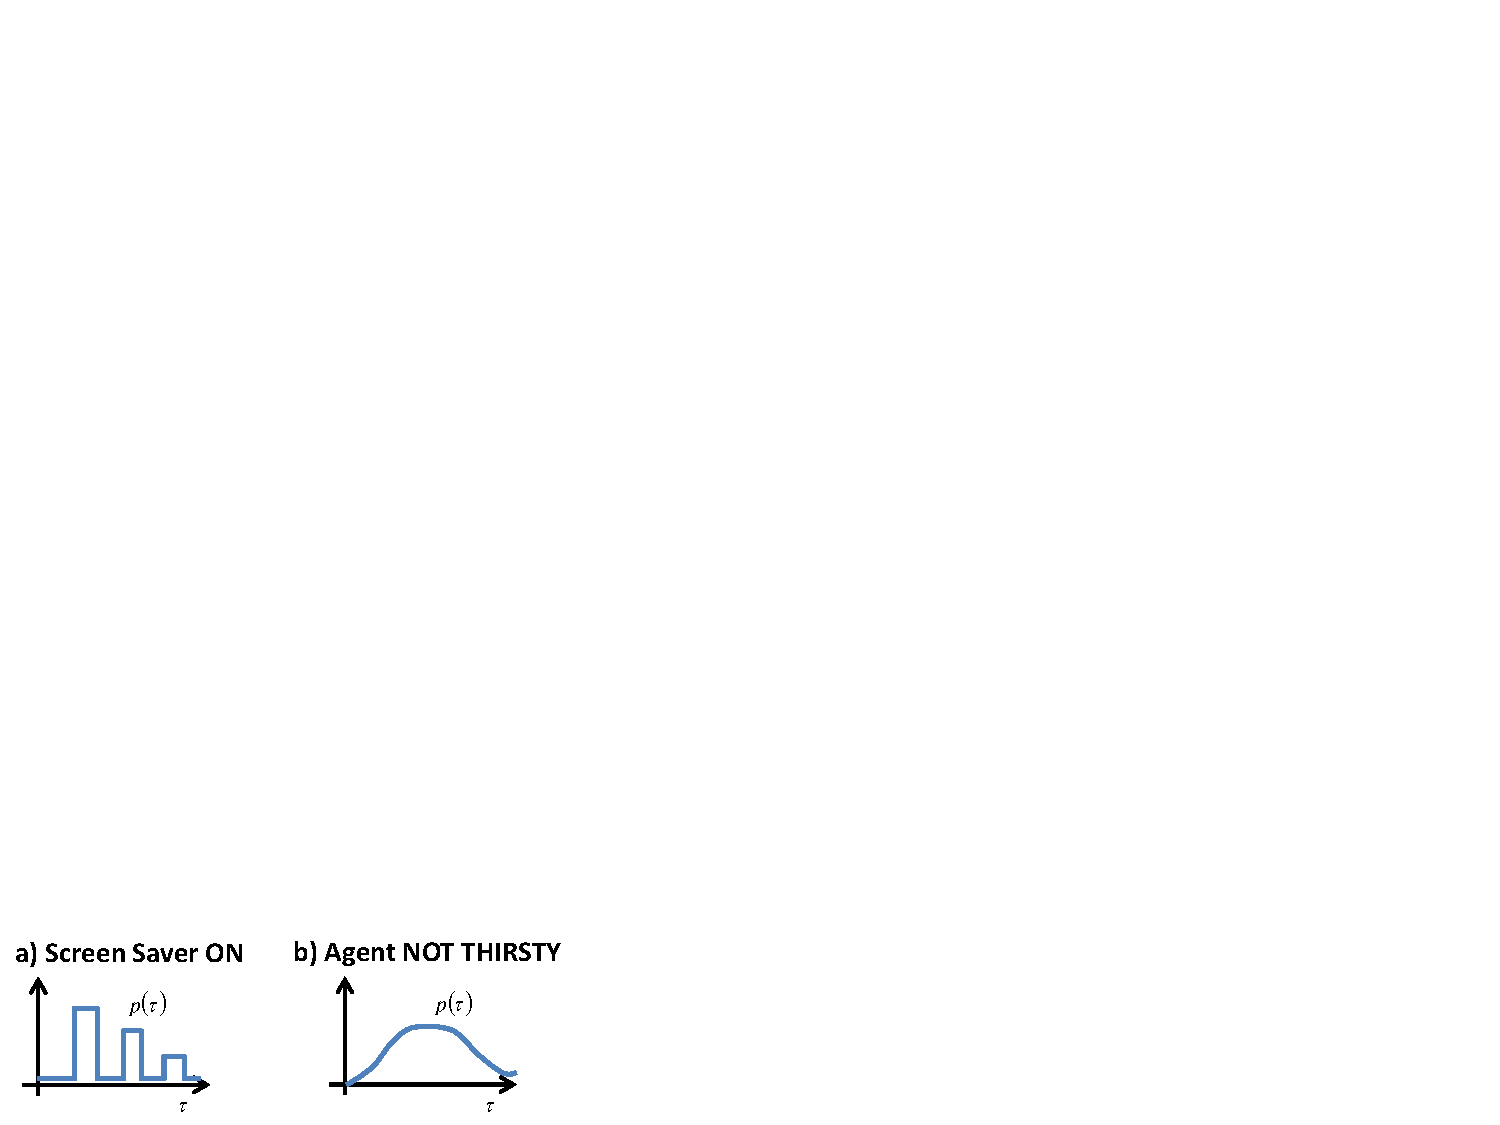
\includegraphics[trim = 0.1in 0.1in 6.25in 6.25in, clip, width=0.9\linewidth]{marginalfi.pdf}
%\fbox{\parbox[c][1in]{2in}{ \centering BLAH }}
\caption{Examples of marginal histograms of durations of $F$. 
TODO: rework with tikz/pgf, make thirst flatter
\label{fig:marginalfi}}
\end{figure}


\todo[inline]{EXPLAIN MORE DETAILS ABOUT SURVIVAL ANALYSIS.  AND WHY EVERY 5 MINUTES HAVE INSTANCE--BECAUSE MICROSOFT SET IT UP THIS WAY.  }

\todo[inline]{BY DEFAULT, HAVE AN INERTIAL PROBABILITY...  HOW LONG THINGS WILL NOT CHANGE. TALK ABOUT THIS CONCEPT.}

Figure~\ref{fig:marginalfi} shows some histograms of durations.  After removing adjusting for when the screensaver remains off due to causal actions such as moving the mouse or using the keyboard, the histogram for the duration the screensaver is off, shown in (a), is mostly discrete.  The histogram was acquired by asking  participants for their screensaver set times.  (TODO: experiment)  Where commonsense knowledge is available, these histograms can be directly coded.  When evidence is available, these distributions can be learned from observation.

For more subjective fluents, such as the thirst of an agent, where limited information is known ahead of time, flatter histograms are used such as that shown in Fig.~\ref{fig:marginalfi}(b).  Uniform histograms are used to model fluents where an agent's action removes any time dependence.

The research presented here extends current causal models of fluents to accommodate consistency constraints and probability distributions on durations.



This research builds on recent progress in action and event recognition.  Event recognition fills in missed or occluded actions through grammar models \cite{Mingtao} or hidden Markov models/dynamic Bayesian networks \cite{Brand, DBN}.  To improve recognition rates for small or challenging objects, joint inference is performed over the context,  taking agent actions together with the objects or parts \cite{yao2010modeling}.  


The research presented in this paper extends the trend of using joint spatial, temporal, and causal inference one step further, using detected actions to infer particular values for fluents and using detected fluent values to confirm or correct action detections.  These inferred values are then used to reason backward and forward in time, providing coherent values for fluents and actions over the course of the video.  For example, an agent filling a cup suggests that the cup lacked water before the action and contains more water after it.

We use the same methods to connect actions to fluents of the mind.  Recent cognitive-science literature has focused on goal inference \cite{Tenenbaum2009Cognition, csibra2007obsessed}, and this framework has been extended to vision research \cite{Mingtao}.  The goal detection presented in \cite{Mingtao} identifies actions as part of a routine, or a larger set of actions, and then information about the routine is used to predict future actions, such as those that would complete the routine.  However, this line of research has so far not explored the larger goal of the routine, such as thirst motivating an agent to obtain and drink water.  Another contribution of the present study is in connecting the larger routines of actions to their triggering fluents through causal reasoning. 



\subsection{Joint inference: Action and fluent interaction}

\todo[inline]{Point out: THIS IS 2-WAY INFORMATION--FROM ACTION TO FLUENTS AND SOMETIMES FLUENT TO ACTION}

\todo[inline]{EXPLAIN FIGURE 1 BETTER (MOVE HERE)... USE THIS EXAMPLE TO EXPLAIN HAVE FLUENT CHANGE, OBSERVED ACTIONS.  MAKE SOME OF FLUENTS OBSERVABLE (NOT ALL HIDDEN).  ADD LIGHT EXAMPLE (INFER SOME ACTIONS: TURN ON LIGHT, WHICH IS NOT OBSERVABLE).  SHOWING 2-WAY STREET.  ADD DASHED DIAMOND TO THE TOP.  }



Each of the fluents thus far described takes a value at each instant of time, allowing the notation $F(t)$ to describe the value the fluent $F$ takes at time $t$.  For example, if $F$ represents the light status, then $F(t) = \textrm{ON}$ indicates that the light is on at time $t$.  

At each instance of time, there is a causal explanation for the fluent value, $F(t)$.  This causal explanation was studied in \cite{morrow2012pami}, and connects $F(t)$ to actions by attributing the fluent value either to a particular action or to a lack of change-inducing action.    Following the light example, the causal explanation could be because an agent just turned the light on or because the light was on and no one turned it off.  

The causal connection between values of fluents and agent actions matches the values of fluents and agent actions in a commonsense way.  This key connection allows inference of hidden fluents and of actions, even when they are not detectable or when they may be detected incorrectly.  

For example, while the action of going to the wall and raising a hand is detectable from video, without labelling the light switch as the object being touched on the wall, it is impossible to tell  that the action is ``flipping the light switch''.  However, an understanding of the cause and effect relationship allows the cause (``flipping the light switch'') to be probabilistically detected (matched the the detected action) once the effect has been detected (light has come on). 

This paper extends methods in \cite{morrow2012pami} to accommodate joint inference, allowing values of fluents to provide feedback in order to inform detections of agent actions.


\subsection{Related work}

\todo[inline]{NEED SEPARATE SECTION DEVOTED TO Related Work}

\todo[inline]{1: PSYCHOLOGY IN CAUSAL INFERENCE.  KEN NAKAYAMA'S WORK (ILLUSORY CAUSAL CRECSCENTS: MISPERCEIVED SPATIAL RELATIONS DUE TO PERCEIVED CAUSALITY)--VISUAL PERCEPTION.}

\todo[inline]{2: COMMONSENSE REASONINING -- USING LOGIC TO REASON, BUT THIS IS TOO FRAGILE.}

\todo[inline]{3: INFER CAUSALITY IN STATISTCS-- PEARL BAYES NET (NOT CONNECTED/GROUNDED TO IMAGES IN VIDEO.}

\todo[inline]{4: EVENT ANALYSIS -- HERE, SAY "WE'RE JUST BUILDING ON THIS ...  MOVE SOME OF THE "BACKGROUND" SECTION HERE.}



\subsection{Summary of contributions}

This paper presents a method for joint temporal-causal inference that allows the coherent inference of fluents for the duration of a video.  

An overview of the joint inference process is shown in Figure~\ref{fig:jointinference}.  Each video is first temporally described with probability.  These descriptions and probabilities are then processed with potential causal explanations, and the best performing causal description is returned.  By following the causal description back to its individual components, hidden actions and values of fluents are determined.  % TODO: i don't mention "dynamic" anywhere here...  where to introduce this term?

\begin{figure}[hbtp]
\centering
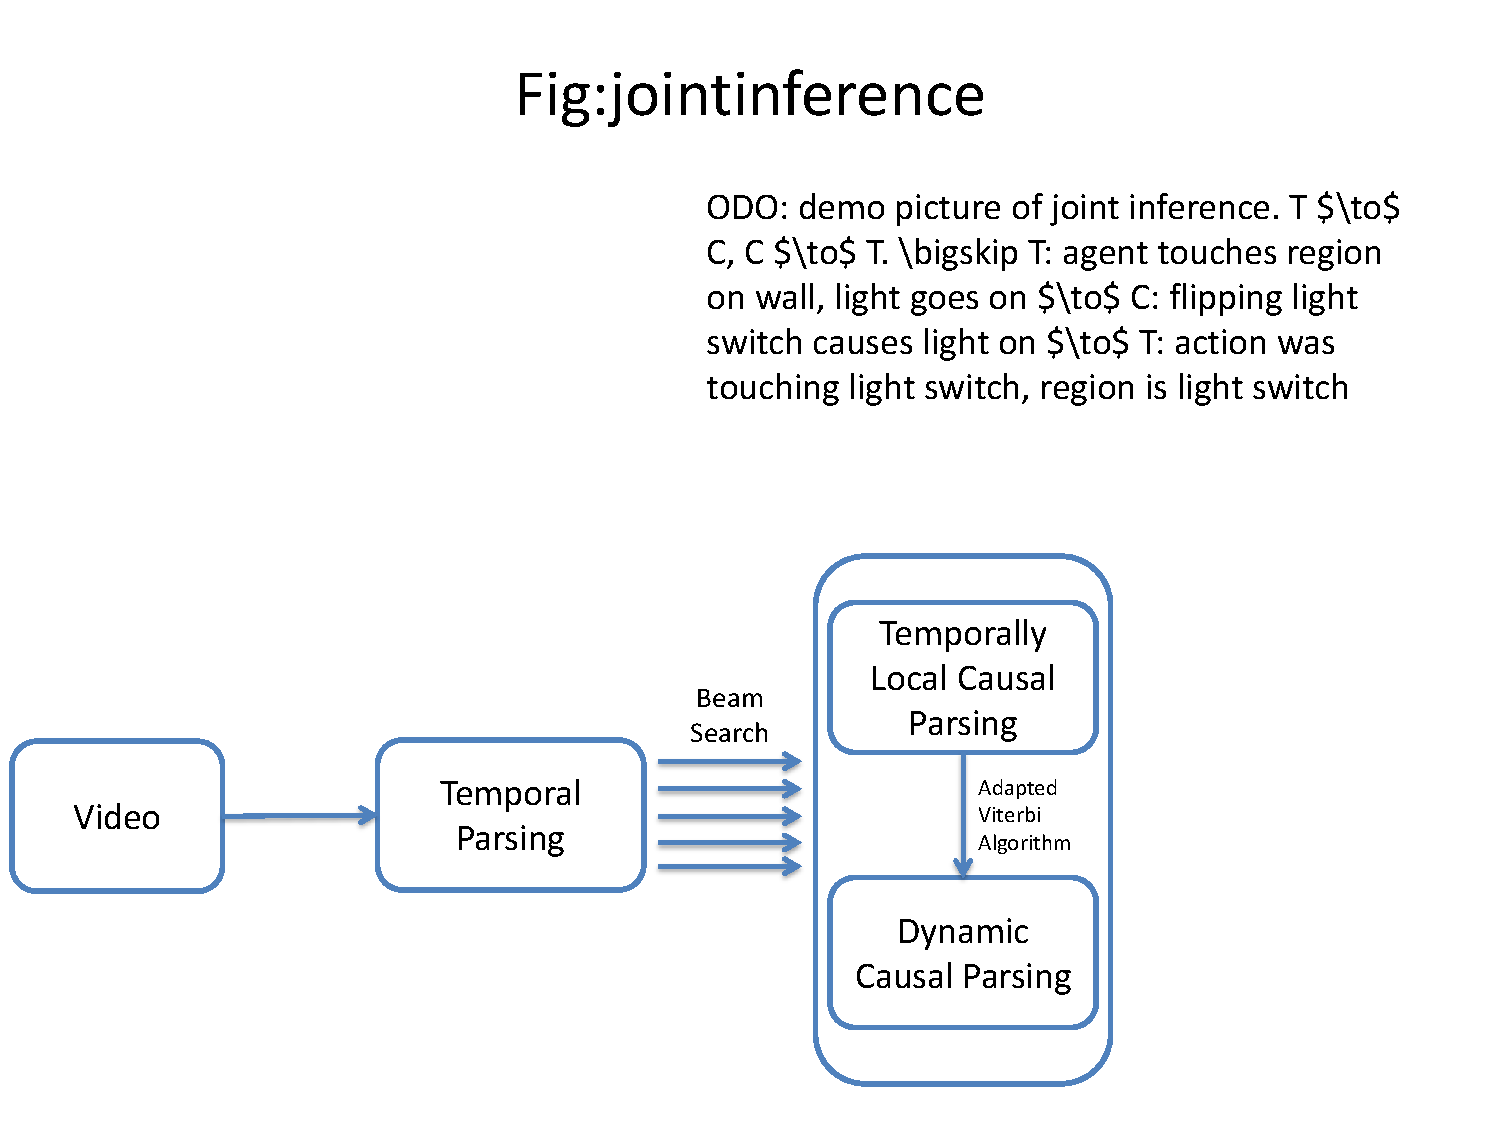
\includegraphics[trim = 0in 0.25in 2.5in 3.5in, clip, width=0.9\linewidth]{jointinference.pdf}
\caption{Joint inference \label{fig:jointinference}}
\end{figure}
%\fbox{\parbox[c][2in]{2in}{ \centering TODO: demo picture of joint inference.  T $\to$ C, C $\to$ T.  \bigskip  T: agent touches region on wall, light goes on $\to$  C: flipping light switch causes light on $\to$ T: action was touching light switch, region is light switch}}


\todo[inline]{CLARIFY FIG 3 FOR MY 2 PARTS: (PARSING ON C-AOG AND DP WITH INSERTION FOR REASONING).  CLARIFY INPUT: 
ASSUME OBSERVED FLUENT CHANGE AND ACTIONS INPUT ARE INDEPENDENT (AT EACH TIME) OF EACH OTHER, WITHOUT INVOLVING TEMPORAL AOG.  OUTPUT: HIDDEN FLUENT INFERRED...  REFER BACK TO FIGURE 1.}


  We summarize our contributions here:
\begin{itemize}
\item Joint inference of fluents and actions.  A model is derived that uses causal information to connect fluents to actions consistently over the duration of a video.  
\item Inference of fluents over time.  The joint model integrates constraints to allow consistent inference of fluents over time.  Algorithms are provided to navigate the solution space.
\item Inference of trigger conditions.  The joint model uses trigger conditions, both of states of the world and of the agent's mind, to provide richer reasoning of fluents in the scene.  %TODO: make sure this is explicit in the model somehow
\item Exploration of human cognition of fluents.  Experiment results that include human judgements enlighten the community about human processing of fluents.  %TODO (decide if claiming this) 
\end{itemize}

\todo[inline]{PARAGRAPH: THE PAPER IS ORGANIZED AS FOLLOWS...}

\section{Background}

Causality is the key connecting actions and fluents (hidden or not) in video.  Causality, as studied by commonsense reasoning and AI researchers, is often formulated in terms of first-order logic \cite{CommonsenseReasoning}.  However, purely deductive methods typically do not allow for probabilistic solutions, which are important in computer vision research where maintaining ambiguity is essential.  While methods exist that allow for probability \cite{MarkovLogicNetwork, PearlCausality}, these methods have not been grounded on vision sensors.  While Bayesian networks are commonly used to represent causality \cite{PearlCausality}, the expressive power of a grammar model can represent a greater breadth of possibilities than a single instance of a Bayesian network \cite{TenenbaumCausalGrammar}, making it more suitable for vision applications.

Further, grammar representations are advantageous over competing Hidden Markov Models (HMM) and Dynamic Bayesian Networks (DBN) for representing events.  By allowing for multiple configurations and high level structures, the hierarchical structure of grammar provides maximum flexibility in representing events in video.    

%Meanwhile, the vision literature on causality is sparse.   Some vision models use causal relationships in event recognition \cite{HakeemShah, Chellappa, PEL}, and others use measures of causality to learn similar patterns of actions in repeated events \cite{TemporalCausality}.  

Grammar models are embodied in the graphical representation of the And-Or Graph (AOG) \cite{HeuristicSearch}.  The AOG was first applied to vision in the spatial domain \cite{StochasticGrammar}, and has since been extended to the represent temporal explanations \cite{Mingtao} and causal relationships \cite{morrow2012pami}.  In the AOG, Or-nodes are used to represent alternatives, and And-nodes are used to represent hierarchical decompositions.  How these nodes are used depends on the context: temporal or causal.

In this section, we introduce the AOG as used for events and causality in this paper.


\subsection{Describing actions: the T-AOG}

\todo[inline]{TALK J(MINIMALLY) ABOUT PARSING, ACTIONS, EVENTS....  JUST HIGHLIGHTING THE INPUT}



Many event parsing techniques use a stochastic grammar with some using context-free and others using context-sensitive.   All these grammars for event parsing can be embodied in the graphical representation of the Temporal And-Or Graph (T-AOG) \cite{Mingtao}, a sample of which is shown in Figure~\ref{fig:taog}.  

In the T-AOG, the And-nodes (solid circles) allow for compositional hierarchy, with events decomposed into subevents, such as the decomposition of action $A_{3}$ into subactions ($a_{31}$ or $a_{32}$), and $a_{33}$.  The Or-nodes (dashed circles) provide alternate configurations, such as the various ways different doors can be unlocked ($a_{31}$ or $a_{32}$).  

At the lowest level, the leaf nodes of the T-AOG represent various relations, from poses of agents to locations of objects and agents.

The T-AOG can be learned in an unsupervised way from video \cite{SiUnsupervisedEvent}.

%\begin{figure}[htbp] 
%\centering
%%\includegraphics[trim = 0.1in 0in 5.4in 4.3in, clip, width=0.9\linewidth]{images/slide78.pdf}
%\fbox{\parbox[c][2in]{2in}{ \centering TODO (after experiments) %: make simplified T-AOG using events also listed in Figure 1.  Include some of Ping's frames at the bottom level to show relationships.  Similar to Fig 6, show one PG darkened.  
%}}
%\caption{A sample T-AOG showing that events are decomposed into subevents and further into actions.  %The bottom-level actions are as follows: $a_{11}$: Push door closed.  $a_{31}$: Unlock with key.  $a_{32}$: Unlock with pass code.  $a_{33}$: Pull door.   $a_{10,1}$: Walk by. $a_{11,1}$: Conversation.  $a_{12,1}$: Pick something up.
%TODO: use tikz/pgf
%\label{fig:taog}}  
%\end{figure}

A parse graph, $pg$, is an instance of the AOG with selections made at the Or-nodes, and provides a high-level interpretation of observed events.  Parse graphs from the AOG of Figure~\ref{fig:taog} are shown over time in Figure~\ref{fig:t_parse_graphs}.  In the T-AOG, fluent changes and causing actions happen independently.  


%\begin{figure}[htbp] 
%\centering
%\fbox{\parbox[c][2in]{2in}{ \centering TODO (after experiments): show the pg extracted }}
%%\includegraphics[trim = 0.4in .1in 4.75in 5.2in, clip, width=0.95\linewidth]{images/t_parse_graphs.pdf}
%\caption{Parse graph from the T-AOG of Figure~\ref{fig:taog} for key actions over time are shown on top, together with fluent changes below.    
%TODO: use tikz/pgf
%\label{fig:t_parse_graphs}}  
%\end{figure}

\todo[inline]{SMOOTH OUT: DITCHED EQUATIONS, ASSUME PROBABILITY IS OUTPUT BY SEQUENCE OF ACTION/CHANGE DETECTIONS.   ASSUME INDEPENDENT DISTRIBUTED.  -- THE LIKELIHOOD.  CITE PAPERS FOR DETECTION.  SIMPLIFY 2.1 A LOT.}

The probability distribution of spatio-temporal parse graphs is a joint probability over the nodes given by 
%\begin{equation} \label{eq:st_probability}
%p_{\mathrm{T}}(pg_{\mathrm{T}}|I) = \frac{1}{z_0} \exp \left( - \mathcal{E_{\textrm{T}}}(pg_{\mathrm{T}}|I) \right)
%\end{equation} 
%where $I$ represents the video (a sequence of images), $\mathcal{E_{\textrm{T}}}(pg_{\mathrm{T}}|I)$ is the total spatio-temporal energy as in \cite{Mingtao} and \cite{StochasticGrammar},
%\begin{equation} \label{eq:st_energy}
%\begin{split}
%\mathcal{E_{\textrm{T}}}(& pg_{\mathrm{T}}|I)  = \sum_{v \in V^{\mathrm{OR}}_T(pg_{\mathrm{T}})}  \lambda_v(w(v)) \\& + \sum_{t \in T(pg_{\mathrm{T}})} \lambda_t (\alpha(t))  
% + \sum_{(i,j)\in R(pg_{\mathrm{T}})} \lambda_{ij} (v_i, v_j),
%\end{split}
%\end{equation}  
and $z_0$ is the normalizing constant.  In $\mathcal{E_{\textrm{T}}}$, $ V^{\mathrm{OR}_T}$ is the set of non-empty Or-nodes in $pg_{\mathrm{T}}$, $T$ is the set of terminal nodes in $pg_{\mathrm{T}}$, and $R$ is the set of temporal relations in $pg_{\mathrm{T}}$.  $T$ consists of atomic actions composed of spatio-temporal relations between objects as well as fluents.  $\lambda_v$, $\lambda_t$, and $\lambda_{ij}$ give potential functions over the respective nodes and relations.  $\lambda_v$ again gives switch probabilities.  For detailed explanation on the T-AOG and the probability distribution, we refer the reader to \cite{Mingtao} and \cite{StochasticGrammar}.  This current work takes these $pg_{\mathrm{T}}$ as input.




\subsection{Representing causality locally: the C-AOG}  
% c-aog only includes action!

\todo[inline]{EXPLAIN MORE.   WHAT IS AND, WHAT IS OR.  LEARNED (CITE MY PAPER).  EXPLAIN HOW MANY PARAMETERS ARE USED IN C-AOG (NOT THAT MANY), HOW ARE THEY DECIDED.  PUT TABLE: HOW MANY CAUSAL EVENTS WE HAVE.}

\todo[inline]{CALL THIS "INSTANTANEOUS", NOT LOCAL}

%%%% For section 2.2, but here for placement issues
\begin{figure*}[hbtp]
\centering
\begin{tikzpicture}[scale=0.5,>=stealth]
\scriptsize
\fill [gray!20] (-2.5,7.5) -- (-2.5,3.5) -- (2,3.5) -- (2,5.5) -- (5,5.5) -- (5,7.5) -- cycle;
\node at (1,7) [label=right:{$F\!=$Display}] {};
\node at (1,6.5) [label=right:{$F_1\!=$Monitor}] {};
\node at (1,6) [label=right:{$F_2\!=$Computer}] {};
\drawFluent{-2}{7}{0.4};\node at (-1.75,7) [label=right:Fluent] {};
\drawAction{-2}{6}{0.4};\node at (-1.75,6) [label=right:Action] {};
\drawInertialAction{-2}{5}{0.4};\node at (-1.75,5) [label=right:Inertial Action] {};
\drawTransitNP{-2}{4}{0.4};\node at (-1.75,4) [label=right:Fluent Transit] {};
%
\draw [->,red!50] (1,0) -- (1.5,1.65);
\draw [->,red!50] (2,0) -- (1.5,1.65);
\draw [->,red!50] (4,0) -- (4.5,1.65);
\draw [->,red!50] (5,0) -- (4.5,1.65);
\draw [->,very thick,red] (7,0) -- (7.5,1.65);
\draw [->,very thick,red] (8,0) -- (7.5,1.65);
\draw [->,red!50] (1.5,2) -- (4.5,3.75);
\draw [->,red!50] (4.5,2) -- (4.5,3.75);
\draw [->,very thick,red] (7.5,2) -- (4.5,3.75);
\draw [->,very thick,red] (10.5,2) -- (11.25,3.75);
\draw [->,red!50] (12,2) -- (11.25,3.75);
\draw [->,very thick,red] (4.5,4) -- (7.875,5.75);
\draw [->,very thick,red] (11.25,4) -- (7.875,5.75);
%
\draw [very thick,red,shift={(7.875,5.75)}] (0,0)+(-150:6mm) arc (-150:-30:6mm);
\draw [red!50,shift={(1.5,1.65)}] (0,0)+(-105:6mm) arc (-105:-75:6mm);
\draw [red!50,shift={(4.5,1.65)}] (0,0)+(-105:6mm) arc (-105:-75:6mm);
\draw [very thick,red,shift={(7.5,1.65)}] (0,0)+(-105:6mm) arc (-105:-75:6mm);
%
\drawFluent{1}{0}{0.4};\node at (1,-1) [] {\parbox{1.5cm}{\centering $F_2(t\!-\!1)\!=$\\AWAKE}};
\drawInertialAction{2}{0}{0.4};
\drawFluent{4}{0}{0.4};\node at (4,-1) [] {\parbox{1.5cm}{\centering $F_2(t\!-\!1)\!=$\\ASLEEP}};
\drawAction{5}{0}{0.4};
\drawFluent{7}{0}{0.4};\node at (7,-1) [] {\parbox{1.5cm}{\centering $F_2(t\!-\!1)\!=$\\ASLEEP}};
\drawAction{8}{0}{0.4};
\drawTransitPP{1.5}{2}{0.4};
\drawTransitNP{4.5}{2}{0.4};
\drawTransitNP{7.5}{2}{0.4};
\drawTransitPP{10.5}{2}{0.4};
\drawTransitNP{12}{2}{0.4};
\drawFluent{4.5}{4}{0.4};\node at (4.75,4) [label=right:{$F_2(t)\!=$AWAKE}] {};
\drawFluent{11.25}{4}{0.4};\node at (11.5,4) [label=right:{\parbox{1cm}{$F_1(t)\!=$\\POWERED}}] {};
\drawHollowFluent{7.875}{6}{0.4}\node at (8.125,6) [label=right:{$F(t)\!=$ON}] {};
\draw [dashed,thick] (5.75,-2.75) [out=90,in=-45] to (5.25,-0.25);
\draw [dashed,thick] (8.75,-2.75) [out=90,in=-45] to (8.25,-0.25);
\node at (5.75,-2.75) [] {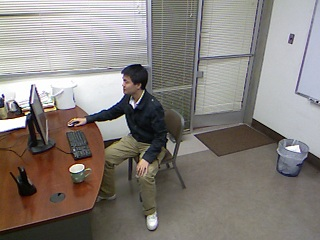
\includegraphics[width=.5in]{185}};
\node at (8.75,-2.75) [] {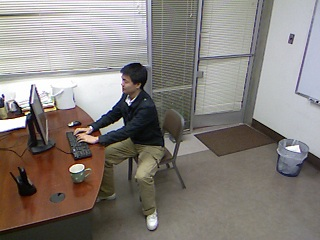
\includegraphics[width=.5in]{275}};
%
\node at (7.875,7) [] {\bf (a) Causal-AOG};
\node at (20,7) [] {\bf (b) Causal-PG};
%
\draw [->,thick] (18,5) -- (24,5);
\draw [thick,cyan] (16,2.75) -- (20,2.75);
\draw [thick,cyan] (20,3.25) -- (24,3.25);
\draw [thick,cyan] (16,0.75) -- (20,0.75);
\draw [thick,cyan] (20,1.25) -- (24,1.25);
\draw [thick,cyan] (16,-0.75) -- (24,-0.75);
\drawAction{18}{5}{0.4};
\node at (20,5.75) [] {Use Keyboard$(t\!-\!1,t_2)$};
\drawFluent{18}{3}{0.4};\drawTransitNP{20}{3}{0.4};\drawFluent{22}{3}{0.4};
\node at (18,2.25) [] {$F_2(t\!-\!1)\!=$ASLEEP};
\node at (22,3.75) [] {$F_2(t)\!=$AWAKE};
\drawFluent{18}{1}{0.4};\drawTransitNP{20}{1}{0.4};\drawFluent{22}{1}{0.4};
\node at (18,0.25) [] {$F(t\!-\!1)\!=$OFF};
\node at (22,1.75) [] {$F(t)\!=$ON};
\drawFluent{18}{-1}{0.4};\drawTransitPP{20}{-1}{0.4};\drawFluent{22}{-1}{0.4};
\node at (18,-1.75) [] {\parbox{1.5cm}{\centering $F_1(t\!-\!1)\!=$\\POWERED}};
\node at (22,-1.75) [] {\parbox{1.5cm}{\centering $F_1(t)\!=$\\POWERED}};
\draw [->,thick] (16,-3) -- (24,-3);\node at (24,-3) [label=below:Time] {};
\draw (18,-2.75) -- (18,-3.25);\node at (18,-3) [label=below:$t\!-\!1$] {};
\draw (22,-2.75) -- (22,-3.25);\node at (22,-3) [label=below:$t$] {};
\node at (15.5,5) [] {\begin{sideways}\parbox{1cm}{\centering Agent\\Action}\end{sideways}};
\node at (15.5,3) [] {\begin{sideways}Computer\end{sideways}};
\node at (15.5,1) [] {\begin{sideways}Display\end{sideways}};
\node at (15.5,-1) [] {\begin{sideways}Monitor\end{sideways}};
%
\draw [->,very thick,red] (18.4,5) -- (19.75,3.25);
\draw [->,very thick,red] (18.25,3) -- (19.6,3);
\draw [->,very thick,red] (20.4,3) -- (21.75,3);
\draw [->,very thick,red] (22,2.75) -- (22,2);
\draw [->,very thick,red] (22,-0.5) -- (22,0.75);
\draw [->,very thick,red] (18.25,-1) -- (19.6,-1);
\draw [->,very thick,red] (20.4,-1) -- (21.75,-1);
\end{tikzpicture}
%\includegraphics[trim = 0in .5in 3.5in .5in, clip, width=.45\linewidth]{causalaog.pdf}
%\includegraphics[trim = 0in .0in 4in 1in, clip, width=.4\linewidth]{causalpg.pdf}
\caption{(a) A C-AOG fragment for the display fluent to take the value ON.  The value of the top level fluent at time $t$, $F(t)$, is a consequence of the values of its children.  Children of And-nodes are connected by arcs.  The fluent transit nodes indicate the kind of change that occurs in the fluent: step functions for change, flat lines for non-change.  The inertial action, a lack of change inducing action, is shown by the non-action symbol.  (b) In the parse graph, selections have been made on the Or-nodes of the C-AOG in (a).  In this case, the display is determined to be on at $t$ because someone used the keyboard, waking the computer.  The monitor's power status (ON) does not change.
TODO: separate this into two figures
 \label{fig:causalpg}}
\end{figure*}

%TODO: emphasize "local"

Identifying agent actions as causes for fluent changes as studied in cognitive science \cite{carey2009origin} and decomposing actions into fluents as used in vision to detect actions \cite{Bobick}, the Causal And-Or Graph (C-AOG) provides a stochastic grammar representation of causality \cite{morrow2012pami}.  This graph integrates with And-Or representations used in vision to represent spatial and temporal knowledge \cite{StochasticGrammar, chen2007rapid, Mingtao}.    

The C-AOG represents a value for a fluent (e.g., $F(t) = \textrm{ON}$ in Figure~\ref{fig:causalpg}(a) where $F$ is the monitor's display state) as a consequence of a temporally local INUS condition, an \textit{insufficient} but \textit{necessary} condition within a set of conditions that is \textit{unnecessary} but \textit{sufficient} for the effect \cite{Mackie}.  In the C-AOG, Or-nodes represent the alternative means of causation (e.g., a monitor, through the computer, can be turned on by someone using a mouse or a keyboard).  And-nodes group causing actions into single INUS conditions.  

A parse graph ($pg$) in the C-AOG, such as that in Figure~\ref{fig:causalpg}(b),  is formed from a selection of the Or-nodes (such as the path shown by thicker, darker lines in (a)).  It provides a causal interpretation for why fluent $F$ has a particular value at time $t$, including fluent values and actions that lead to $F(t)$, as deemed relevant by the C-AOG..  

Most frequently, the most probable causal parse graph for a given fluent at a given time is the inertial parse graph---the fluent maintained its value in the absence of a change-inducing action---such as shown in Figure~\ref{fig:causalpg}(b) for the monitor power status.


\todo[inline]{EXPLAIN THIS EQUATION BETTER.  }

In \cite{morrow2012pami}, the C-AOG is learned in an unsupervised manner by linking actions from the T-AOG to fluents in the spatial domain.  The probability model over the parse graphs available from the C-AOG builds on top of that of the T-AOG and is also defined through the energy.  In particular, $p(pg_\mathrm{C}) = \frac{1}{Z} \exp\left( -\mathcal{E}\left(pg_\mathrm{C} \right) \right)$ where 
\begin{equation}
\mathcal{E}(pg|I)  = \sum_{t=1}^n   \left(\mathcal{E}_{\mathrm{T}}(pg_t|I) + \sum_{v \in V_{\mathrm{C}}^{\mathrm{Or}}(pg_t)} \lambda_v(w(v))\right) .
\end{equation}
$\mathcal{E}_{\mathrm{T}}(pg_t|I)$ is the detection energy from event parsing for the included actions/fluents.  $V_{\mathrm{C}}^{\mathrm{Or}}$ is the set of included Or-nodes in each local $pg_t$, $w(v)$ returns the selected branch, and $\lambda_v$ gives the switch probability on the Or-nodes for the alternative causes as learned by maximum likelihood estimation.  This Or-contribution to the energy specifies a prior on causality that favors the inertial action.  

As we have now discussed two different parse graphs, we include the legend in Table~\ref{tab:pgs} for referencing the parse graph notation over the next few sections.

\begin{table}[htp]
\centering
\caption{Legend of Parse Graph Notation}
\begin{tabular}{rp{2in}}
$pg_\mathrm{T}$ & temporal parse graph \\
$pg$ & causal parse graph \\
$\mathbf{PG}$ & sequence of causal parse graphs, $(pg_1, \ldots, pg_n)$ \\
$pg_t(f_i, f_j)$ & the causal parse graph (explanation) at time $t$ where the fluent value at time $t-1$ was $F(t-1) = f_i$ and the fluent value at $t$ is $F(t) = f_j$
\label{tab:pgs}
\end{tabular}
\end{table}



%Local c-aog fragments: Or probabilities on C-AOG.  Constraint:
%\begin{equation}
%E_{P} \left( h \left( w(v) \right) \right) = h_{v}^{obs}
%\end{equation}


\section{Reasoning: The dynamic C-AOG}

\todo[inline]{CALL OUT CONNECTION TO DYNAMIC BAYES NET (TRANSFER BETWEEN C-AOG, LIKE THEY TRANSITION BETWEEN BAYES NETS)}


%%%% placed here to display on correct page
\begin{figure*}[htp]
\centering
\begin{tikzpicture}[scale=0.5,>=stealth]
\scriptsize
\fill [gray!20] (-6,-2.25) rectangle (-3,2);
\drawAction{-5.5}{1.5}{0.25};\node at (-5.25,1.5) [label=right:Action] {};
\drawHiddenFluent{-5.5}{0}{0.3};\node at (-5.25,0) [label=right:\parbox{1cm}{Hidden\\Fluent}] {};
\drawCausalLink{-5.5}{-1.5}{0.25};\node at (-5.25,-1.5) [label=right:\parbox{1cm}{Causal\\Link}] {};
\fill [gray!20] (4,-1) rectangle (8,-0.25);\fill [gray!20] (4,-2) rectangle (8,-1.25);
\fill [gray!20] (10,-1) rectangle (14,-0.25);\fill [gray!20] (10,-2) rectangle (14,-1.25);
\fill [cyan!20] (11.25,-1) rectangle (11.75,-0.25);\fill [cyan!20] (11.5,-2) rectangle (12.5,-1.25);
\draw [cyan,very thick,dotted] (11.25,-1) -- (11.5,-1) -- (11.5,-0.25) -- (11.75,-0.25);
\draw [cyan,very thick,dotted] (11.5,-1.25) -- (11.75,-1.25) -- (11.75,-2) -- (12.25,-2) -- (12.25,-1.25) -- (12.5,-1.25);
\fill [cyan!20] (16,-1) rectangle (20,-0.25);\fill [cyan!20] (16,-2) rectangle (20,-1.25);
\draw [cyan,very thick,dotted] (16,-1) -- (17.5,-1) -- (17.5,-0.25) -- (19,-0.25) -- (19,-1) -- (20,-1);
\draw [cyan,very thick,dotted] (16,-1.25) -- (17.75,-1.25) -- (17.75,-2) -- (18.25,-2) -- (18.25,-1.25) -- (20,-1.25);
\node at (0,2.5) [] {\bf (a) Input: Video/XML};\draw [->,very thick] (2.5,2.5) -- (3.5,2.5);
\node at (6,2.5) [] {\bf (b) Event Parsing};\draw [->,very thick] (8.5,2.5) -- (9.5,2.5);
\node at (12,2.5) [] {\bf (c) Causal Parsing};\draw [->,very thick] (14.5,2.5) -- (15.5,2.5);
\node at (18,2.5) [] {\bf (d) Causal Completion};
\node at (-0.75,0.25) [] {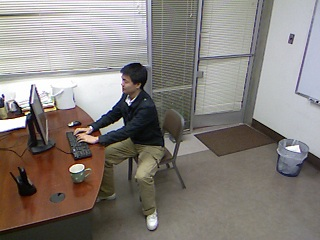
\includegraphics[width=.75in]{275}};
\node at (-0.5,0) [] {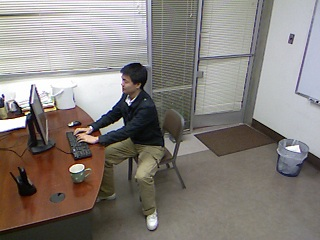
\includegraphics[width=.75in]{275}};
\node at (-0.25,-0.25) [] {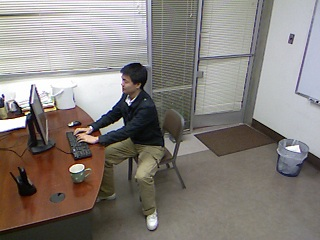
\includegraphics[width=.75in]{275}};
\node at (0,-0.5) [] {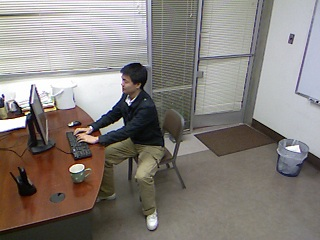
\includegraphics[width=.75in]{275}};
%
\drawHiddenFluent{2.75}{-0.5}{0.3};\node at (4.35,-0.4) [label=left:{\tiny ON}] {};\node at (4.35,-0.9) [label=left:{\tiny OFF}] {};\node at (2.75,0) [] {\tiny Monitor};
\drawHiddenFluent{2.75}{-2}{0.3};\node at (4.35,-1.4) [label=left:{\tiny THIRSTY}] {};\node at (4.35,-1.9) [label=left:{\tiny NOT}] {};\node at (2.75,-2.5) [] {\tiny Agent};
\node at (6,-0.65) [] {UNKNOWN};
\node at (6,-1.65) [] {UNKNOWN};
%
\draw [gray,thick] (6,2) -- (5,1.25);
\draw [gray,thick] (6,2) -- (6,1.25);
\draw [gray,thick] (6,2) -- (7,1.25);
\draw [gray,thick] (5,1.25) -- (4.5,0.5);
\draw [gray,thick] (5,1.25) -- (5.5,0.5);
\drawAction{6}{2}{0.25};
\drawAction{5}{1.25}{0.25};
\drawAction{6}{1.25}{0.25};
\drawAction{7}{1.25}{0.25};
\drawAction{4.5}{0.5}{0.25};
\drawAction{5.5}{0.5}{0.25};
\node at (6,0) [] {\tiny Use Keyboard};
\node at (6.5,0.75) [] {\tiny Drink};
\draw [thick] (4,-2.5) -- (5,-2.5);
\draw [->,thick] (6.5,-2.5) -- (8,-2.5);
\node at (5.75,-2.5) [] {Time};
%
\draw [gray,thick] (12,2) -- (11,1.25);
\draw [gray,thick] (12,2) -- (12,1.25);
\draw [gray,thick] (12,2) -- (13,1.25);
\draw [gray,thick] (11,1.25) -- (10.5,0.5);
\draw [gray,thick] (11,1.25) -- (11.5,0.5);
\drawAction{12}{2}{0.25};
\drawAction{11}{1.25}{0.25};
\drawAction{12}{1.25}{0.25};
\drawAction{13}{1.25}{0.25};
\drawAction{10.5}{0.5}{0.25};
\drawAction{11.5}{0.5}{0.25};
\draw [->,red,very thick] (11.5,0.25) -- (11.5,-0.25);
\draw [->,red,very thick] (11.75,-1.25) [out=90,in=-90] to (12,1);
\draw [->,red,very thick] (12,1) [out=-90,in=90] to (12.25,-1.25);
\draw [thick] (10,-2.5) -- (11,-2.5);
\draw [->,thick] (12.5,-2.5) -- (14,-2.5);
\node at (11.75,-2.5) [] {Time};
%
\draw [gray,thick] (18,2) -- (17,1.25);
\draw [gray,thick] (18,2) -- (18,1.25);
\draw [gray,thick] (18,2) -- (19,1.25);
\draw [gray,thick] (17,1.25) -- (16.5,0.5);
\draw [gray,thick] (17,1.25) -- (17.5,0.5);
\drawAction{18}{2}{0.25};
\drawAction{17}{1.25}{0.25};
\drawAction{18}{1.25}{0.25};
\drawAction{19}{1.25}{0.25};
\drawAction{16.5}{0.5}{0.25};
\drawAction{17.5}{0.5}{0.25};
\draw [->,red,very thick] (17.5,0.25) -- (17.5,-0.25);
\draw [->,red,very thick] (17.75,-1.25) [out=90,in=-90] to (18,1);
\draw [->,red,very thick] (18,1) [out=-90,in=90] to (18.25,-1.25);
\draw [thick] (16,-2.5) -- (17,-2.5);
\draw [->,thick] (18.5,-2.5) -- (20,-2.5);
\node at (17.75,-2.5) [] {Time};
%
\draw (20.25,2.25) -- (20.5,2.25) -- (20.5,0.25) -- (20.25,0.25);
\draw (20.25,0) -- (20.5,0) -- (20.5,-2) -- (20.25,-2);
%
\node at (21,1.25) [] {\begin{sideways}Agent Actions\end{sideways}};
\node at (21,-1.25) [] {\begin{sideways}Fluents\end{sideways}};
\end{tikzpicture}
%\includegraphics[trim = 0in 0in 0in 5.25in, clip, width=.99\linewidth]{flowchart.pdf}
\caption{Overview of the causal reasoning process using dynamic C-AOGs.  For simplicity, only the monitor's display status and agent's thirst status are shown.  (a) Event parsing results of a video are used as input.  (b) Standard event parsing leaves many fluent values unassigned over the duration of the video.  (c) Causal parsing assigns causal links between actions and fluents, allowing some fluent values to be filled in as preconditions or effects of agent actions.  (d) Causal completion using the dynamic C-AOG fills in the fluents for the remaining times.  TODO: change "causal completion" to "dynamic causal parsing"
 \label{fig:flowchart}}
\end{figure*}

%TODO: decide on notation for parse graphs, and write the constraints in terms of it.


While the C-AOG as described above, referred to henceforth as a ``local C-AOG fragment'', represents the causal relations of a fluent at a single instant of time (using actions and conditions in a small window around that time), it lacks a mechanism to bind these instances forward and backward in time.  Over the course of a sequence of events, however, knowing the fluent values at key points enables reasoning about the values of the fluents throughout the whole video sequence.  Figure~\ref{fig:flowchart} summarizes this reasoning process.  %For example, when a cause-inducing action occurs, the fluent changes value, but in the absence of such an action, the fluent maintains status.  The duration over which the fluent maintains its value is governed by the duration of the inertial action (the lack of change-inducing action).  
This section introduces the dynamic C-AOG for binding the temporally local C-AOG fragments together and for modeling the duration of the inertial action (when the fluent maintains status).


%%%%% for placement with section 3.2
\begin{figure*}[htp]
\centering
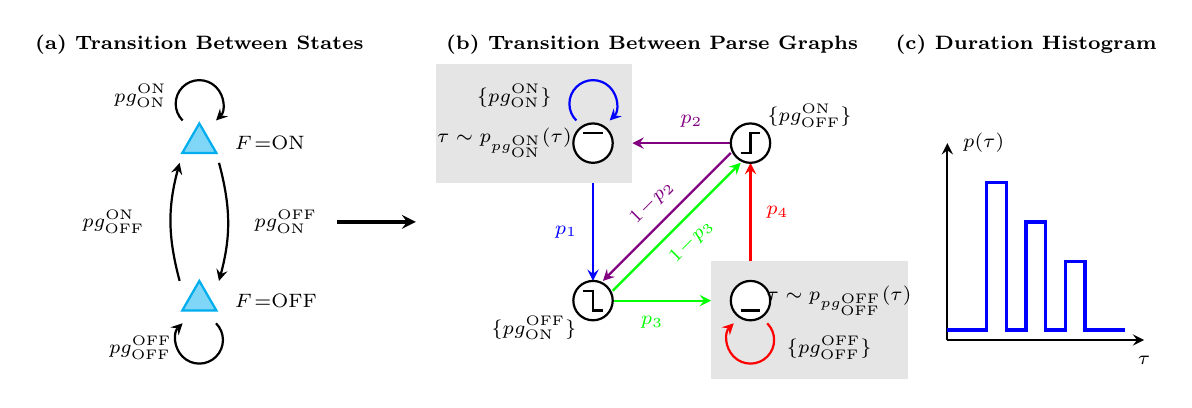
\begin{tikzpicture}[scale=0.5,>=stealth]
\scriptsize
\node at (1,7.5) [] {\bf (a) Transition Between States};
\node at (12.5,7.5) [] {\bf (b) Transition Between Parse Graphs};
\node at (22,7.5) [] {\bf (c) Duration Histogram};
%
\drawFluent{1}{1}{0.5};\node at (1.5,1) [label=right:{$F\!=$OFF}] {};\node at (-0.5,0.5) [label=below:{$pg_{\text{OFF}}^{\text{OFF}}$}] {};
\drawFluent{1}{5}{0.5};\node at (1.5,5) [label=right:{$F\!=$ON}] {};\node at (-0.5,5.5) [label=above:{$pg_{\text{ON}}^{\text{ON}}$}] {};
\draw [->,thick] (1.5,4.5) [out=-75,in=75] to (1.5,1.5);\node at (0,3) [label=left:{$pg_{\text{OFF}}^{\text{ON}}$}] {};
\draw [->,thick] (0.5,1.5) [out=105,in=-105] to (0.5,4.5);\node at (2,3) [label=right:{$pg_{\text{ON}}^{\text{OFF}}$}] {};
\draw [->,thick,shift={(1,0)}] (0,0)+(45:6mm) arc (45:-225:6mm);
\draw [->,thick,shift={(1,6)}] (0,0)+(225:6mm) arc (225:-45:6mm);
%
\draw [->,very thick] (4.5,3) -- (6.5,3);
%
\draw [->,thick,violet] (15,5) -- (12,5);\node at (13.5,5) [label=above:{\color{violet}$p_2$}] {};
\draw [->,thick,green] (11,1) -- (14,1);\node at (12.5,1) [label=below:{\color{green}$p_3$}] {};
\draw [->,thick,blue] (11,4) -- (11,1.5);\node at (11,2.75) [label=left:{\color{blue}$p_1$}] {};
\draw [->,thick,red] (15,2) -- (15,4.5);\node at (15,3.25) [label=right:{\color{red}$p_4$}] {};
\draw [->,thick,green] (11.5,1.25) -- (14.75,4.5);\node at (13.5,2.5) [rotate=45] {\color{green}$1\!-\!p_3$};
\draw [->,thick,violet] (14.5,4.75) -- (11.25,1.5);\node at (12.5,3.5) [rotate=45] {\color{violet}$1\!-\!p_2$};
%
\fill [gray!20] (7,7) rectangle (12,4);
\fill [gray!20] (14,2) rectangle (19,-1);
\drawTransitPP{11}{5}{0.5};\draw [->,thick,shift={(11,6)},blue] (0,0)+(225:6mm) arc (225:-45:6mm);\node at (9,5.5) [label=above:{$\{pg_{\text{ON}}^{\text{ON}}\}$}] {};\node at (8.75,5) [] {$\tau\sim p_{pg_{\text{ON}}^{\text{ON}}}(\tau)$};
\drawTransitPN{11}{1}{0.5};\node at (9.5,1) [label=below:{$\{pg_{\text{ON}}^{\text{OFF}}\}$}] {};
\drawTransitNN{15}{1}{0.5};\draw [->,thick,shift={(15,0)},red] (0,0)+(45:6mm) arc (45:-225:6mm);\node at (17,0.5) [label=below:{$\{pg_{\text{OFF}}^{\text{OFF}}\}$}] {};\node at (17.25,1) [] {$\tau\sim p_{pg_{\text{OFF}}^{\text{OFF}}}(\tau)$};
\drawTransitNP{15}{5}{0.5};\node at (16.5,5) [label=above:{$\{pg_{\text{OFF}}^{\text{ON}}\}$}] {};
%
\draw [->,thick] (20,0) -- (25,0);\node at (25,0) [label=below:$\tau$] {};
\draw [->,thick] (20,0) -- (20,5);\node at (20,5) [label=right:$p(\tau)$] {};
\draw [very thick,blue] (20,0.25) -- (21,0.25) -- (21,4) -- (21.5,4) -- (21.5,0.25) -- (22,0.25) -- (22,3) -- (22.5,3) -- (22.5,0.25) -- (23,0.25) -- (23,2) -- (23.5,2) -- (23.5,0.25) -- (24.5,0.25);
\end{tikzpicture}
%\includegraphics[trim = 0in 2in 0in 2.5in, clip, width=.95\linewidth]{transitions.pdf}
\caption{(a) For a given set of values that a fluent can take (here, ON and OFF), the transitions between values also define the transitions between the parse graphs.  (b) The dynamic C-AOG governs the transition between parse graphs by adding two features to the temporally local C-AOG fragments: a limitation on the available parse graphs and a duration capability for maintaining a given status.  (c) Durations for maintaining status are sampled from histograms.  In this histogram, the monitor is on and the most likely durations until a screensaver comes on are in even increments (such as multiples of 5 minutes).
TODO: grey boxes...  the set notation labels the node, the probability should label the arrow...  switch!  also, change notation to pg(ON, OFF), etc.
 \label{fig:transitions}}
\end{figure*}


\todo[inline]{3.1, 3.2: EXPLAIN THE DURATION TERMS AND CONSISTENCY TERMS}]	

\subsection{Model formation and types of constraints}

\todo[inline]{SET UP BACKGROUND FOR NEXT SECTION (INFERENCE).}

\todo[inline]{TRANSITION PROBABILITY --  HOW LIKELY TRANSITIONS BY ITSELF.  }

It is assumed that the observed fluents and actions in a given video sequence follow an underlying probability distribution, $f$, on $\mathbf{PG}$, the sequence $(pg_1, pg_2, \ldots, pg_n)$ of temporally local causal explanations at each timepoint of the video $i = 1, \ldots, n$.  

While the distribution $f(\mathbf{PG})$ is unknown, it can be approximated with a model $p$ by matching constraints to the observed data.

To initialize the process, the method takes observations from the distribution $p_0$ on local C-AOG fragments.  In this paper, we fit two types of constraints: consistency terms, and duration histograms.

We first present the constraints used, and then we derive the dynamic C-AOG model, $p$, by matching the model to the data on the constraints.





\subsection{Consistency constraints on local C-AOG fragments}

\todo[inline]{CLARIFY!!!! MAYBE MOTIVATE THESE CONSTRAINTS WITH THE DIAGRAM FOR C-AOG. } 

%GIVEN THESE CONDITIONS, THEN CERTAIN FLUENTS CHANGE WITH PROBABILITY NEARLY 100\% (WITH PROBABILIY 1, IT'S GOING TO CHANGE).  ALMOST LIKE CONDITION ON ACTION, HAVE TRANSITION PROBABILITY ON THESE FLUENTS.  SUPPOSE OBSERVE ACTION, THIS CHANGES TRANSITION PROBABILITY OF THE FLUENT.  OBSERVE FLUENT CHANGE, INFER BACKWARD CAUSE THE FLUENT CHANGE.  ]]

%[[IN EQUATION BELOW, SHOULD HAVE PROBABILTY OF FI, FJ | A, DURATION.  COULD SIMPLIFY THINGS. IF NO ACTION, GIVEN MORE TIME, HAVE TRANSITION PROBABILITY.  REMOVE HIERARCHY OF ACTIONS.  TRIVIALIZE C-AOG TO INSTANTANEOUS, TO MAKE IT INTO CONDITIONAL PROBABILITY (GIVEN ACTION).  ]]

As shown in Figure~\ref{fig:transitions}(a), a fluent transitions between values over time; the temporally local C-AOG fragments explain why each of these transitions occurs.  At $t-1$, $t$, and $t+1$, the fluent $F$ transitions between values $F(t-1) = f_i$, $F(t) = f_j$,  and $F(t+1) = f_k$.  At $t$ and $t+1$, the transitions are causally described by local C-AOG fragments, $pg_t (f_i, f_j)$ and $pg_{t+1} (f_j, f_k)$ respectively.  This transition between states also describes a transition between the local C-AOG parse-graph fragments, where the parse graph at $t+1$ is chosen from 
\begin{equation}
 \{pg (f_i, f_j) \} = \{pg : F(t) = f_j, F(t+1) = f_{i} \}, 
\end{equation}
which is a subset set of all the parse graphs for $F$. 

\todo[inline]{earlier... describe what all parse graphs for $F$ look like (in particular, those for ON, those for OFF, etc)}

This transition gives rise to the first kind of constraint, the consistency constraint.  For any two parse graphs, $pg (f_i, f_j)$ and $pg(f_k, f_l)$, let $h_{C}$ calculate the consistency between the two as follows
\begin{equation}
h_{C} \left( pg (f_i, f_j), pg(f_k, f_l) \right) = \delta \left( f_j = f_k \right)  = \begin{cases} 1, \textrm{ if } f_j = f_k \\ 0 , \textrm{ otherwise}, \end{cases}  
\end{equation}
where $\delta \left( f_j = f_k \right)$ is the Dirac delta function.

In particular, the expected value under the model, $E_{p}$, for each transition between subsequent parse graphs, $pg_{t}$ and $pg_{t+1}$, is therefore given by
\begin{equation} E_{p} \left( h_C (pg_{t}, pg_{t+1}) \right) = 1. \end{equation}
This constraint must hold for each $t = 1, \ldots, n-1$, giving a total of $n-1$ consistency constraints.

% TODO: derive the gibbs term for the lambda...  make sure jives with what i think

The process of transition between the parse graphs is illustrated in Figure~\ref{fig:transitions}(b), where $F(t)$ has two possible values, ON and OFF, and each node is a temporally local parse-graph fragment from the C-AOG, such as shown in Figure~\ref{fig:causalpg}(b).  Following the consistency constraint, a parse graph of the type $pg(\textrm{ON}, \textrm{ON})$ can only transition to a parse graph of the form $pg(\textrm{ON}, \textrm{ON})$ or $pg(\textrm{ON}, \textrm{OFF})$.  

The consistency constraints thus far described ensure a coherent solution to the reasoning process by limiting the way subsequent local parse graphs can be connected. 



\subsection{Duration constraints}

To detect hidden fluents over long periods of time, the naive approach patches the temporally local C-AOG fragments together according to spatio-temporal detections, using only the consistency constraints thus far described.  While this restricts the parse graphs available for time $t+1$, problems still arise.  If action detections produce inconsistent fluent values, how to resolve the inconsistencies is unclear.  In the naive approach, there is no way to specify whether it is more likely that a hidden change occurred between the two (and when that change occurred), or one of the detections was incorrect.  For example, without knowledge of screensaver settings, it is unidentifiable whether the monitor display switches to screensaver automatically, after a specified period of time, or never.  It is also necessary to represent an internal timer for the hidden fluents of the mind, such as an agent eventually developing thirst.  Including a probabilistic timer mechanism to model the duration can fix these problems with the naive approach.

The standard solution of using a Markovian process to connect local parse graph fragments does not work in this case.  A typical memoryless Markovian process, in which the transition probabilities are constant, leads to exponential fall-off for maintaining one state.  Considering the monitor display fluent duration histogram shown in Figure~\ref{fig:transitions}(c), one can see how unreasonable the exponential fall-off is for fluents.

Therefore, transitions between the parse graphs representing different values for a fluent must be represented more generally than either the naive approach or a typical memoryless Markov process allow.  Duration constraints are used to model how long a fluent can maintain a particular value, which is closely tied to the duration for which the inertial parse graph explains the fluent values.  The process is illustrated in the grey boxes of Figure~\ref{fig:transitions}(b).  

The duration constraints can take many forms, depending on the fluent.  Below, we include a couple of examples of the constraints used for fluents in this paper, classified by their familiar resulting maximum entropy distributions.  Let $\tau$ represent the duration a fluent, $F$, takes a given value, $f$.  

\textbf{Piecewise uniform}.  For fluents such as the screensaver, histograms were collected such as that shown in Figure~\ref{fig:marginalfi}(a).  In this case, it was found that people set screensavers around five minute increments.
% (TODO: correct based on experiments)  
After correcting for parse graphs with causing actions performed by agents, the duration a screensaver is off is modeled by the histogram shown.  On each interval, $I_i$, with constant probability, the boolean for whether $F$ repeatedly takes value $f$ for a duration of $\tau$ within interval $I_i$ is 
\begin{equation}
h_{D, I_i} (\tau) = \delta(\tau \in I_i)
\end{equation}
where $i$ indexes the intervals.  This gives a sequence of constraints where 
\begin{equation}
E_p \left( h_{D, I_i} (\tau) \right) = p_i,
\end{equation}
where $p_i$ is the probability the duration falls in the respective section of the piecewise uniform distribution.  For the screensaver, the constraints are given by the probabilities on the intervals, including $\varepsilon$ around each five minute increment.

\textbf{Uniform}.  For fluent values with no time dependence observable in the video (e.g., the light turning on/off), the uniform distribution is used to eliminate any importance of the duration.  Even though the duration for an agent's thirst does not follow a uniform distribution, the uniform is justifiably used since the videos studied here are not long enough to warrant an expected pattern in agent's thirst.  

The process of remaining in a local parse graph fragment is visualized in the grey boxes of Figure~\ref{fig:transitions}(b), where the duration is selected following a distribution $p(\tau)$.

The duration constraints described allow the consideration of seemingly inconsistent subsequent parse graphs by providing a mechanism for inserting a spontaneous change of the fluent value.  We next combine the duration and consistency constraints with the distribution of the local C-AOG fragments in a single probability distribution.

% TODO: note: screensaver.  it will always be the same one.  BUT.  thirst is more variable.  so somehow this is selecting a model.  and then matching histograms on that model?



\section{Learning}
%\subsection{Minimum KL-divergence distribution}

\todo[inline]{DERIVE THE EQUATIONS/ENERGY (AND EXPLAIN PARAMETERS).  CORRESPOND EACH TERM TO A STATISTICAL OBSERVATION FROM THE PREVIOUS SECTIONS (SECTION 3).}

\todo[inline]{MAYBE: DITCH C-AOG FOR NOW (AND JUST GO WITH CONDITIONAL PROBABILITY...  $\Delta F | A$.}

\todo[inline]{INTRODUCE TRANSITION PROBABILITY.  EITHER OBSERVATION OF STATUS CHANGE.  SOME ARE INPUT, SOME ARE LEARNED THROUGH CAUSAL AOG LEARNING PROCESS.  }

\todo[inline]{POSS: IF ACTION HAPPENS, CHANGES TRANSITION PROBABILITY.  IF THOSE 2 KIND OF TRANSITION PROBABILITIES CANNOT EXPLAIN THE FLUENT CHANGE (DURATION CANNOT EXPLAIN LIGHT ON/OFF), THE PROBABILITY TOO LOW/ZERO, THEN IT MUST INSERT THE ACTION THERE SO THAT TRANSITION HAPPENS.  MAY SIMPLIFY INFERENCE SECTION...  OVER TIME, FLUENT CHANGE BY ITSELF, FINE.  THEY HAVE CERTAIN TRANSITION PROBABILITIES.  IF THAT TRANSITION PROBABILITY IS REALLY REALLY LOW, OR IMPOSSIBLE, BUT IT STILL HAPPENS, THEN JUST SAY MUST INSERT ACTION THERE.  SO HAVE \textbf{PRIOR PROBABILITY THERE TO PENALIZE INSERTING ACTIONS}.  BUT GET REWARDED BY TRANSITION PROBABILITY.  SO ALL I NEED IS TO SPECIFY THE STATUS PGI AND THE TRANSITION BETWEEN THEM.  THEN THE WHOLE THING BECOMES DP, AND I'M DONE.  OF COURSE, THE DP IS MOTIVATED BY ANOTHER PROCESS (DENY OR INSERT A NEW INPUT)  }

\todo[inline]{POSS: TRIVIALIZE CAOG INTO CONDITIONAL PROBABILITY, GIVEN ACTION OR NOT.  THEN: 
CAN STILL HAVE C-AOG FOR FLUENT CHANGE BEFORE/AFTER.  WHEN OBSERVE CERTAIN ACTION.  THEN NEED TO KNOW THE FLUENT.  DRINK CUP, INFER CUP HAD WATER.  FOR THIS NEED C-AOG.  }








Each $pg_t$ from a local C-AOG fragment causally explains the status for a single time $t$, and the sequence, $\mathbf{PG} = (pg_1, pg_2, \ldots pg_n)$, from the dynamic C-AOG explains the video.  

%TODO: include local caog fragment constraints...

Beginning with a distribution over the spatio-temporal parse graphs, $p_{\textrm{ST}}$, a model $p$ is selected from $\Omega_p$, the set of all models fitting the constraints listed above.  Among all such $p$, the model closest to $p_{\textrm{ST}}$ is selected, as measured by the KL-divergence.  That is, $p$ is selected such that 
\begin{equation}
p = \textrm{argmin} KL(p || p_{\textrm{ST}}). \label{eq:minkl}
\end{equation}
This method is the extension of the maximum entropy principle, where the reference distribution would be uniform.  Equation~\ref{eq:minkl} produces a model of the form 
\begin{equation}
p(\mathbf{PG} | I) = \frac{1}{Z} p_{\textrm{ST}} (\mathbf{PG} | I) \exp \left( \sum_{\textrm{constraints} } \lambda_i h_i(\mathbf{PG} | I) \right).
\end{equation}
where $I$ represents the video (sequence of images), the $\lambda_i$ are Lagrange multipliers, and $Z$ is the normalizing constant.  The constraints are used to solve for the $\lambda_i$.  


This gives rise to an energy that is decomposed in terms of the durations, consistencies, and local C-AOG fragments:
\begin{equation}
\begin{split}
\mathcal{E}(\mathbf{PG}|I)  & = \underbrace{\sum_{\tau} \mathcal{E}_D(\tau)}_{\textrm{duration}} + \underbrace{\sum_{t = 2}^n \mathcal{E}_C(pg_{t-1} , pg_{t})}_{\textrm{consistency}} + \\ 
& \sum_{t=1}^n  \underbrace{ \left(\mathcal{E}_{\mathrm{T}}(pg_t|I) + \sum_{v \in V_{\mathrm{C}}^{\mathrm{Or}}(pg_t)} \lambda_v(w(v))\right) }_{\textrm{local C-AOG fragments}} ,
\label{eq:dynamicenergy}
\end{split}
\end{equation}
%TODO: clean up that energy, add appropriate lambdas (maybe)

\textbf{Local C-AOG fragments.}  Given the durations and the transitions, the temporally local parse graph fragments are independent. 

\textbf{Duration.}  The duration terms enforce a timer for fluents that do not have causing actions by trying to add an event to explain a misperceived, or a spontaneous, change. 

\textbf{Consistency.}  Because a single local C-AOG fragment contains the fluent values at $t$ and $t-1$, constraints are required to ensure coherence between subsequent local fragments.  The consistency term is a hard constraint. 

The probability, $p$, on $\mathbf{PG}$ causally describes the changes of the fluent jointly over time.  Where the naive approach selects the value of a fluent based only on its value at the previous time, $p$ allows reference to history beyond one step.



\subsection{Visualizing the probability: The dynamic C-AOG}

The graphical representation of the energy in Equation~\ref{eq:dynamicenergy} is given by the dynamic C-AOG, as shown in Figure~\ref{fig:transitions}(b).  The dynamic C-AOG incorporates the temporal-duration terms together with restrictions on the types of parse graphs available, controlling the selection of the local C-AOG parse graphs.   Each node of the dynamic C-AOG is a temporally local causal parse graph.  The dynamic C-AOG provides a graphical mechanism to visualize the transitions between these local parse graphs.



\subsection{The joint causal/temporal AOG}

The energy term in Equation~\ref{eq:dynamicenergy} depends on the ST-energy provided.  This ST-energy and parse graph pair provided through temporal parsing can consist of a single pair maximum or many pairs with a full distribution over ST-parse graphs.  In the latter case, the energy allows joint selection of the optimal ST-parse graphs jointly with the causal explanations.  

In the next section, we provide algorithms for inferring parse graphs in both situations.



\section{Inference algorithm}

\todo[inline]{EXPLAIN WHERE TO INSERT, AND WHEN, AND WHICH ONE.  }



The optimal sequence, $\mathbf{PG}$, explaining the video is causally provided by 
\begin{equation}
\mathbf{PG} = \textrm{argmax}_{\mathbf{PG}} P(\mathbf{PG|I}).
\end{equation}
Inference is performed by capitalizing on the long durations of inertial parse graph due to the infrequency of action and fluent information from event parsing.  Starting with parse graphs and energies from event parsing, a set of potential causal explanations is first constructed by calculating energies for relevant temporally local C-AOGs.  These potential fragments are then propagated over time, using an adaptation of the Viterbi algorithm.  The compatible sequences of potential fragments are output, along with their energies.

The inference algorithm seeks to optimize the energy function in Equation~\ref{eq:dynamicenergy} by adapting the traditional Viterbi algorithm to accommodate the non-Markovian duration terms.  The temporally local causal parse graphs form the hidden state nodes that the traditional Viterbi algorithm would navigate over.  Departing from the traditional Viterbi algorithm, the algorithm presented here includes a nested minimization within each step.  This minimization attempts to insert a spontaneous change due to the duration term, if such is warranted, and is illustrated in Figure~\ref{fig:inferencealgorithm}.  We begin by first formalizing the adapted Viterbi algorithm, and then we provide methods for the joint inference of causal and temporal parse graphs.

\begin{figure}[htp]
\centering
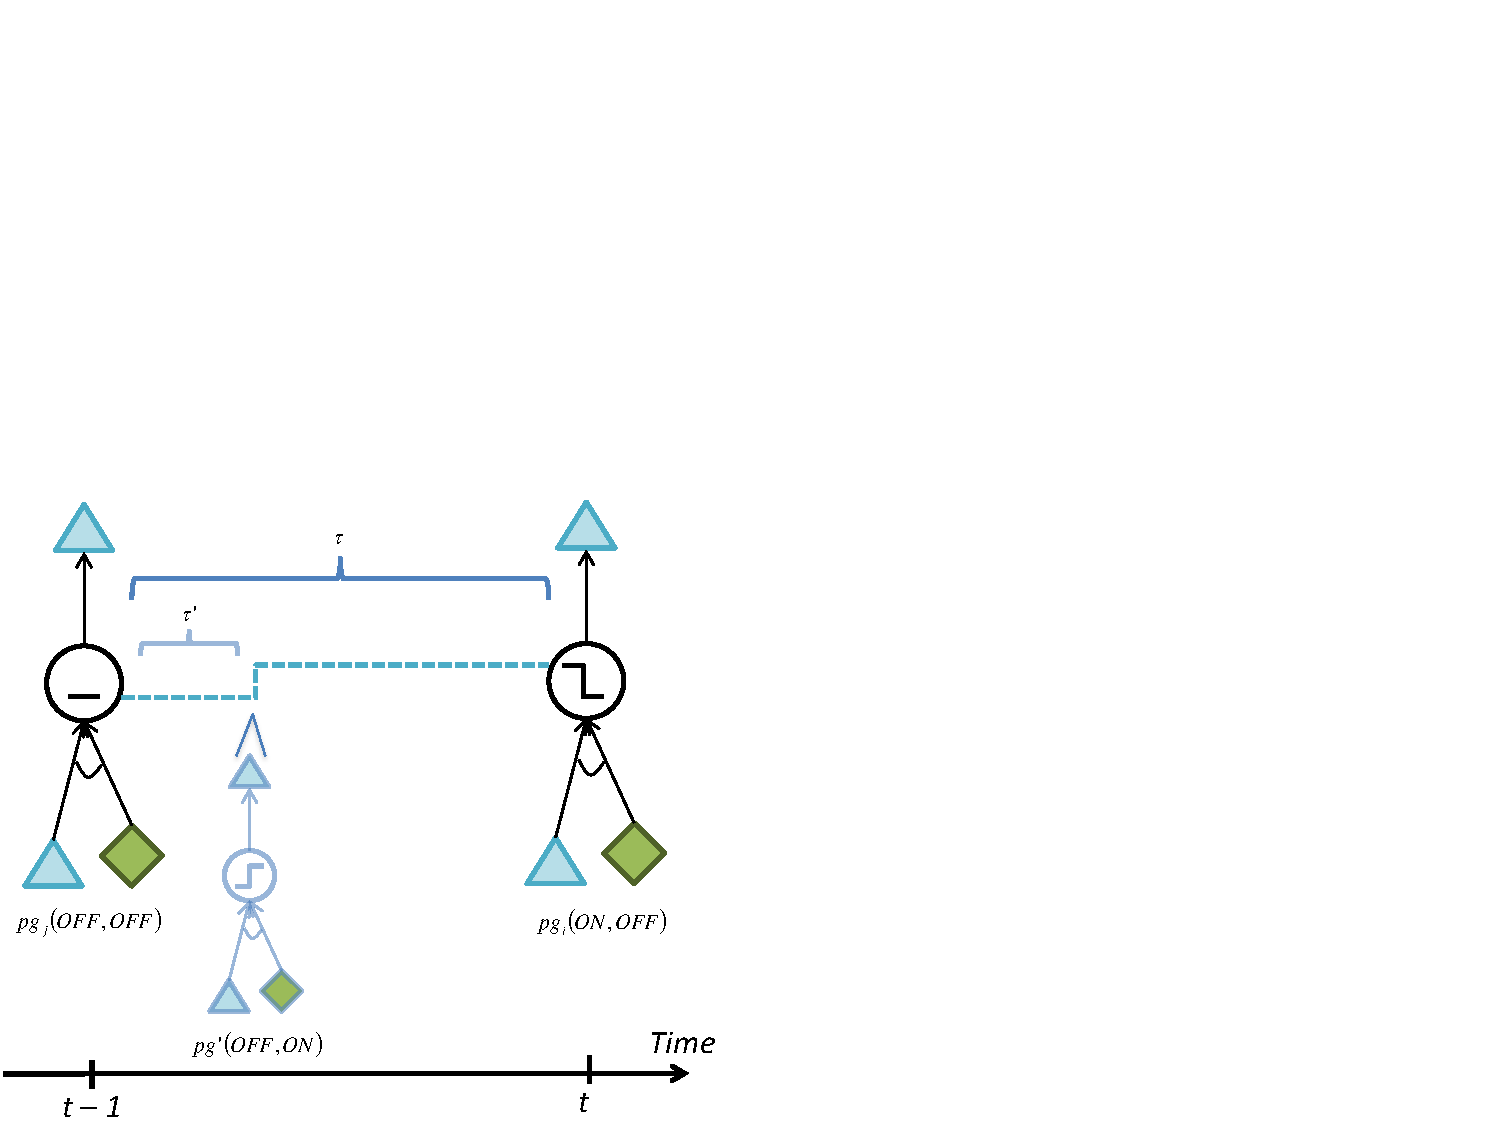
\includegraphics[trim = 0in 0in 5.25in 3.25in, clip, width=.9\linewidth]{inferencealgorithm.pdf}
\caption{Insertion step of inference algorithm, exampled on the screensaver fluent. The Viterbi algorithm tries to find optimal subsequent parse graphs based on the temporally local and consistency energy contributions.  Before accepting the new energy of the parse graphs connecting the two important time points, a new parse graph is optimally inserted between them.  If the insertion improves the energy, the insertion is kept.  This process promotes chains that would otherwise be inconsistent where the duration constraint warrants, and can demote seemingly consistent chains that violate duration constraints.
TODO: make pretty in tikz
\label{fig:inferencealgorithm}}
\end{figure}

%TODO: make it so that if uniform duration, duration term doesn't affect things.



\subsection{Assumptions}

We begin by only examining ``important'' time points, that is, time points where either a change in a fluent or a causing action is detected.  This reduces the necessary search space. In general, all instances between these important time points are best explained by the causal parse graph with the inertial action: the fluent maintains status because no change-inducing action occurred.   For simplicity, these so-called important time points are numbered consecutively, indexed with $t$.

The one exception to the generalization regarding the parse graphs  between important time points occurs when a ``spontaneous'' change is instigated due to the duration term.  That is, the duration term can be responsible for a change in fluent values for a given fluent, $F$, between those time points.  We make the additional assumption that the duration term can be responsible for at most one change in fluent values for $F$ between those time points.  This assumption is reasonable for the fluents studied here, where a spontaneous change happens for only one of the fluent values in those cases.  For example, there is a perceived spontaneous change to ON for the screensaver when no agent is using the computer, but only actions can turn the screensaver OFF.  Similarly, an agent's thirst appears to be turned ON spontaneously, but OFF is activated by drinking.

These two assumptions reduce computation time, and allow for a more efficient algorithm.  By only examining important time points, we reduce the search space for the algorithm.  Further, by limiting the number of spontaneous fluent changes, we are able to adapt the Viterbi algorithm for the non-Markovian process, as we develop in the next section.
% TODO: transition better



\subsection{Adaptation of the Viterbi algorithm}

% TODO: cite viterbi algorithm

Our adaptation of the Viterbi algorithm finds the most likely sequence of local C-AOG fragments that results in the given sequence of input ST-parse graphs, shown in Figure~\ref{fig:viterbialgorithm}.

\begin{figure}[htp]
\centering
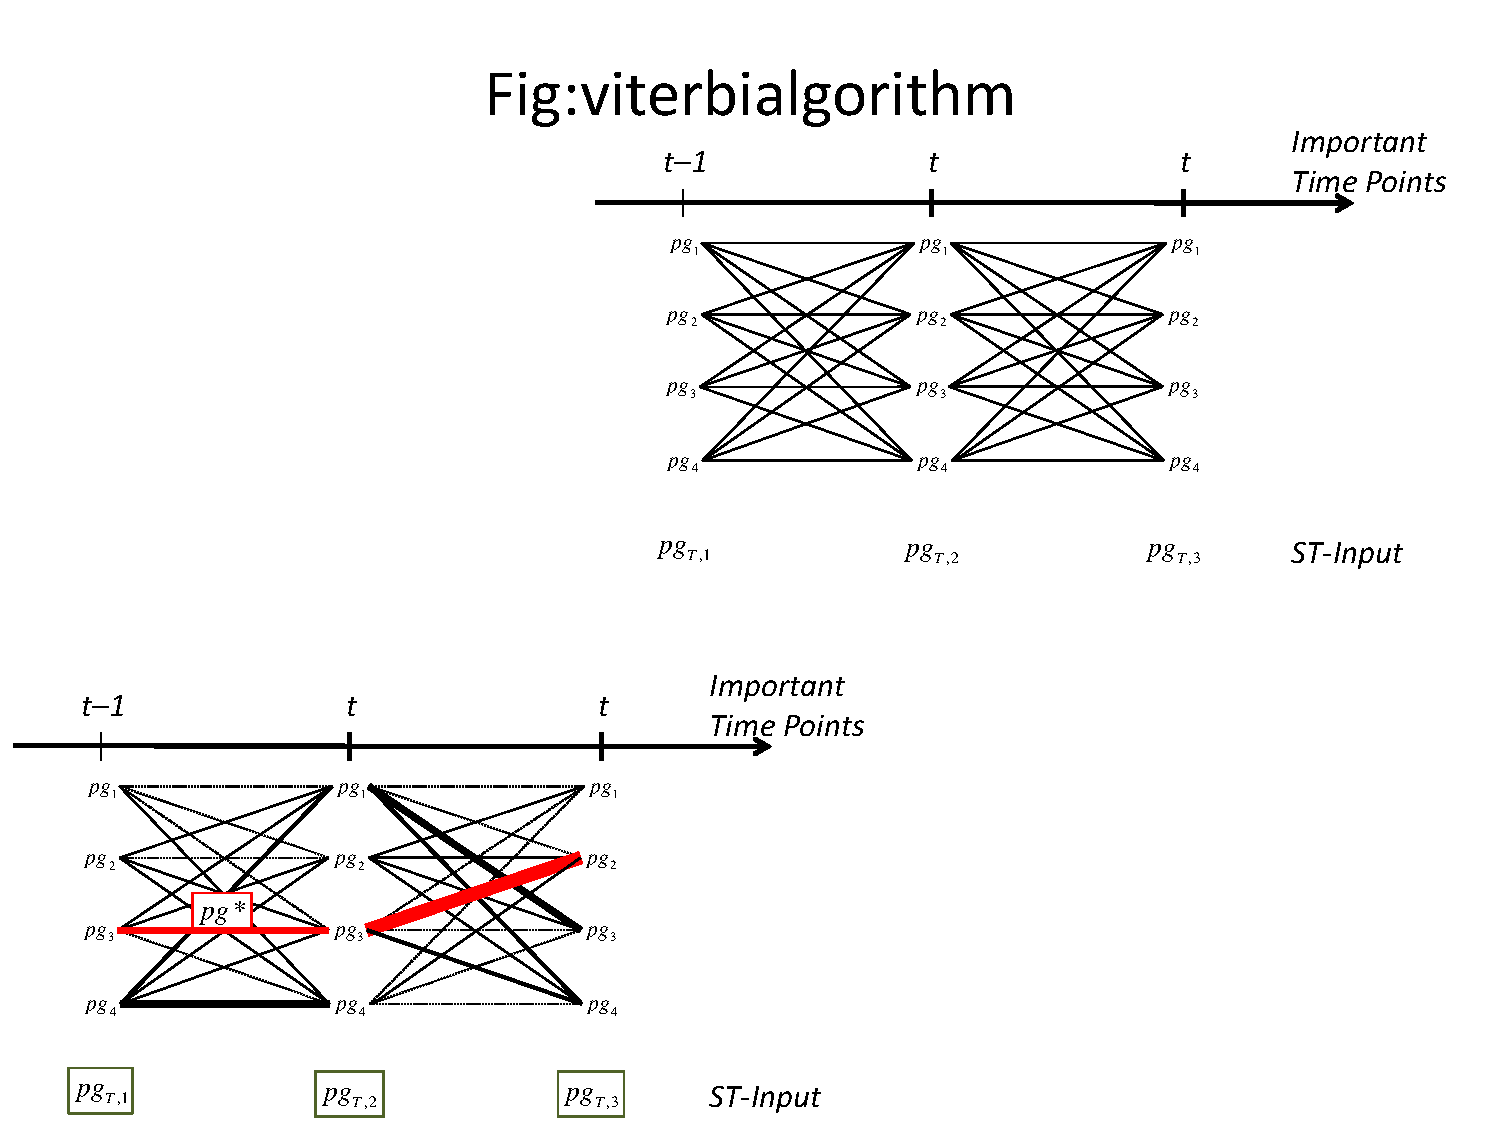
\includegraphics[trim = 0in 0in 4.25in 4.5in, clip, width=.9\linewidth]{viterbialgorithm.pdf}
\caption{The adapted Viterbi algorithm.  The most probable path is computed recursively.  Here, the path includes a local C-AOG fragment inserted because of the energy contribution of the duration terms.  % TODO: more caption
TODO: make pretty in tikz
\label{fig:viterbialgorithm}}
\end{figure}

Given the local parse graph fragment at important time point $t-1$ and the duration the fluent has maintained state due to the inertial action, the energy of the most probable path to the next important time point, $\delta_t$, is recursively given by
%\begin{equation}
%\delta_t(pg_i) = \max_{pg_j} \left( \delta_{t-1}(pg_j) p(pg_i | pg_j, \tau (pg_j) ) p(I | pg_j) \right), 
%\end{equation}
%with the corresponding most probable parse graph at $t$ given by
%\begin{equation}
%\phi_t(pg_i) = \mathrm{argmax}_{pg_j} \left(\delta_{t-1}(pg_j) p(pg_i | pg_j, \tau (pg_j) ) \right).
%\end{equation}
%
\begin{equation}
\delta_t(pg_j, \tau) = \min_{pg_i} \left( \delta_{t-1}(pg_j) + \mathcal{E}(I | pg_j)+  \mathcal{E}^{*}(pg_i, pg_j, \tau )  \right), 
\end{equation}
where $\mathcal{E}(I | pg_j) $ is the observation energy described in \ref{sec:observation_energy} and $\mathcal{E}^{*}(pg_i, pg_j, \tau )$ is the energy from duration and consistency constraints described in \ref{sec:e_star}.  The recursion is initialized with the energies from the temporally local fragments at the first important time point.



\subsubsection{Energy contribution from the local C-pg}
\label{sec:observation_energy}

The third term, $\mathcal{E}(I | pg_j)$, is the energy resulting from parsing on the temporally local C-AOG fragments.  The local C-AOG contribution to the energy of Equation~\ref{eq:dynamicenergy} consists of a ST-energy from the ST-parsing process and a prior energy.  These energies add to form the local C-AOG energy.

When a fluent change or an action is detected (i.e., at an important time point), the energies are examined for all potentially relevant local C-AOG fragments.  Local fragments are deemed relevant if (a) they contain the action or fluent in question as one of their nodes, or (b) they have the same top-level fluent as those already included.  % TODO: maybe explain why

If the fluent change is detected before the action, it is assumed that the causing action must have already occurred or that the fluent change was mis-detected.  Both cases thus require the consideration of all local parse graph fragments with the same top-level fluent.  In this case, all relevant local parse graphs are completed:  energies are tallied (using a prior when there is no detection information), the fluent change is considered irrelevant to the future, and the relevant local parse graphs are considered as the hidden state nodes for the time point.  

If the action is detected first, however, new important time points are continually considered until the distance in time exceeds a pre-set latent time.  The latent time is set based on the fluent, and ``instantaneous'' fluents have the shortest latent times.  If the fluent change is detected within the latent time, all parse graphs for the top-level fluent are completed as explained above.  If the fluent change is not detected before the latent time runs out, then the local parse graphs are completed at the end of the latent time, and the action is considered dealt with.  

These completed parse graphs form the states for each important time point that is tracked throughout the adapted Viterbi algorithm.  Parsing on the local C-AOG fragments provides competing $pg$ to causally explain each fluent change and/or action at the important time point.  %Consecutive $pg$ are enumerated with indices $i$ and $j$ in the next step.

%TODO: include this formalization:
%For a given fluent $F$ with temporally local parse graph fragments $\{ pg(a,b) \}$, the local parse graph fragments define the state space for the fluent. 
%Elements comprising the sequence $\mathbf{PG}$ are selected from $\{ pg(a,b) \}$.   %TODO: needs a time dependence term




\subsubsection{Energy from duration and consistency constraints}
\label{sec:e_star}

The nested minimization, $\mathcal{E}^{*}$, incorporates the consistency terms, and attempts to insert a spontaneous event. $\mathcal{E}^{*}$ compares the effect on the energy of such an insertion between two local parse graphs at consecutive important time points, $pg_i(a,b)$ and $pg_j(c,d)$.  

The proposed insertion considers the duration that the fluent has maintained the value $b$, weighing possible inconsistencies against the length of duration.  We let $\tau$ denote the amount of time the sequence has thus far maintained fluent value $b$.  In particular, if $a \ne b$, then $pg(a,b)$ represents a change in fluent, and $\tau  = 0$.  However, if $a = b$, then $\tau  > 0$.

\todo[inline]{POSS: CHANGE TO BE AS A  MONTECARLO JUMP. BEFORE INSERT, HAVE STATUS A; AFTER INSERT, GO TO STATUS B.  STATUS A AND B HAVE DIFFERENT ENERGIES.  ACCEPT WITH PROBABILITY. }

Under an insertion, the lowest possible energy depends on the consistency contributions, as well as duration contributions before and after the insertion:
\begin{equation}\begin{split}
\mathcal{E}^{*}_I = \min_{\substack{ \tau' < \tau \\ pg'}} & \left(  \underbrace{ \mathcal{E}_C  (pg_{i}(a,b), pg') + \mathcal{E}_C (pg', pg_j(c,d))}_{\textrm{Consistency}} \right. \\ 
& +\underbrace{\mathcal{E}_D (\tau') + \tau' \mathcal{E}(pg_{\mathrm{Inert}} (b,b))}_{\textrm{Before Insertion}} \\
& \left. +\underbrace{ \mathcal{E}_D (\tau - \tau')+ (\tau - \tau') \mathcal{E} (pg_{\mathrm{Inert}} (c,c))}_{\textrm{After Insertion}} \right).
\end{split}
\label{eq:e_star_i}
\end{equation}
where $\mathcal{E}_C$ and $\mathcal{E}_D$ are the energies from Equation~\ref{eq:dynamicenergy}.  $pg_{\mathrm{Inert}} (b,b)$ is the non-action inertial parse graph maintaining fluent value $b$.  $\tau$ is tracked from the end of the last non-action parse graph, and is only relevant at the start of the next non-inertial parse graph.

Without an insertion, on the other hand, 
\begin{equation}
\mathcal{E}^{*}_{NI} =  \mathcal{E}_C (pg_{i}, pg_j)  + \mathcal{E}_D (\tau) +\tau \mathcal{E}(pg_{\mathrm{Inert}} (b,b)) .
\label{eq:e_star_ni}
\end{equation}

$\mathcal{E}^{*}$ is then computed
\begin{equation}
\mathcal{E}^{*}  = \min\left(\mathcal{E}^{*}_I, \mathcal{E}^{*}_{NI} \right)
\label{eq:e_star}
\end{equation}
When there is no significant duration term, this reduces to
\begin{equation}
\mathcal{E}^{*} = \mathcal{E}^{*}_{NI}.
\end{equation}


%Calculate $\mathcal{E}(pg_i | pg_j, \tau (pg_j) )$: If $\tau(pg_j) > 0$, then subtract the energy contribution in the last part.  Calculate if it is desirable to try to add a ``spontaneous'' event.  Note: because assuming at most 1 unexplained change possible, need to check if a change hurts energy for consistent pg's, and need to check if a change improves energy for inconsistent ones (thereby smoothing the inconsistency).  If the inconsistency is improved, add the optimal placement of the change to the list of important time points.  If fluent value maintains, energy contribution is for acquiring a duration at least that long (which is why the subtraction happens).  If time/space require, dispose of chains that have near zero probability.  TODO: CLARIFY!!!


If $\mathcal{E}^{*} = \mathcal{E}^{*}_{I}$, then the best temporal location to insert a parse graph, along with the best inserted parse graph is given by:
\begin{equation}
\label{eq:phi_star}
\phi^{*}_t(pg', \tau') = \mathrm{argmin}_{pg', \tau'} \left( \mathcal{E}^{*}(pg_i, pg_j, \tau ) \right). % TODO: fix subscript on argmin  ...  http://tex.stackexchange.com/questions/5223/command-for-argmin-or-argmax
\end{equation}

%TODO: i reversed order of i and j at some point.  go back and make sure i caught all of them!

Further, the corresponding most probable parse graph at $t$ given by
\begin{equation}
\label{eq:phi}
\phi_t(pg_j) = \mathrm{argmin}_{pg_i} \left(\delta_{t-1}(pg_j) + \mathcal{E}^{*}(pg_i, pg_j, \tau ) \right). 
% TODO: fix subscript on argmin  ...  http://tex.stackexchange.com/questions/5223/command-for-argmin-or-argmax
\end{equation}







%Maybe reclassify duration term as duration to unexplained/hidden change. 

%Actually don't need to consider events not happening. This happens automatically because I complete all pg. need to add in the one that I have no evidence for too. If not doing that already. 




%Currently
%\begin{itemize}
%\item temporal/spatial parsing result: fluent values at times (for known fluents), and event parse graphs with times.  
%\item get all causal pg's possible where action or fluent change occured (the rest are due to inertial).  time event completed considered important for causal parsing.
%\item make all possible chains.
%\item select chain with highest probability
%\end{itemize}
%

% ATTEMPTING THE ALGORITHM
%taking one from each parse competing class:
%1. pg a b. 2  pg c d. 3 pg e f.  
%duration $\sim \tau$
%
%take 1 and 2.
%if compatible
%	check duration. (if duration relevant)
%	if duration has high probability, 
%		great.
%	else
%		attempt to insert event/change of fluent TODO
%else  ( not compatible)
%	attempt to insert event/change of fluent
%
%return a valid chain part and its probability	.  or remove combination.  uh-oh...  this means we might want to look at keeping one or the other.  bah.
%
%attempt to insert event/change of fluent

The preceding equations give rise to the inference algorithm for the dynamic C-AOG.  This algorithm is summarized in Algorithm~\ref{algo:causalinference}.


% TODO: change to algorithmicx package
% Inference Algorithm
\LinesNumbered
\begin{algorithm}[htb]
\SetKwInOut{Input}{Input}\SetKwInOut{Output}{Output}
\small
\Input{ST-pg from video, and probabilities}
\Output{Most probable sequence of C-pg}
\BlankLine
\ForEach {important time point $t$}
{
	Complete all temporally local causal parse graphs\;
	\If{$t > 2$}
	{
		Calculate $\mathcal{E}^{*}_{I}$, $\mathcal{E}^{*}_{NI}$, and $\mathcal{E}^{*}$ according to Equations~\ref{eq:e_star_i}, \ref{eq:e_star_ni}, and \ref{eq:e_star}\;
		Create hashes by Equations~\ref{eq:phi} and \ref{eq:phi_star}\;
	}
}
Return lowest energy (most probable) $\mathbf{PG}$\;
\caption{Dynamic causal inference}\label{algo:causalinference}
\end{algorithm}


\subsection{Joint inference}

Joint temporal and causal inference is performed through a beam search over the temporal parse graphs.  The top performing temporal parse graphs are used, one at a time,  as input for the dynamic causal parsing process of Algorithm~\ref{algo:causalinference}.  This added step is summarized in Algorithm~\ref{algo:jointinference}.   

\LinesNumbered
\begin{algorithm}[htb]
\SetKwInOut{Input}{Input}\SetKwInOut{Output}{Output}
\small
\Input{Sequence of top $n$ ST-pg from video, and probabilities}
\Output{Jointly most probable sequence of T-pg and C-pg}
\BlankLine
%Tally observations\;
%Initialize model estimates\;  %Prepare the examples
\ForEach {ST-pg}
	{
	   Compute most probable sequence of C-pg by Alg.~\ref{algo:causalinference}\;
	}
Return the overall most probable $\mathbf{PG}$\;
\caption{Joint temporal and causal inference}\label{algo:jointinference}
\end{algorithm}




   
   

\section{Consequences of inference}

While the main output of the inference is to find the jointly most probable temporal and causal explanation of the observed events and fluents, the inference process described can be used in deeper ways.

\subsection{Special fluents: preconditions, trigger conditions, and relative fluents}

Using the dynamic C-AOG, causal explanations are used to reason hidden fluent values throughout the video.  This section describes how the capacity of the dynamic C-AOG is expanded by adding three new types of fluents to the local C-AOG fragments: preconditions, trigger conditions, and relative fluents.

The local C-AOG fragments can be extended to include key fluent preconditions for a richer description of the causing state.  The original C-AOG only considered agent actions as INUS causing conditions.  However, by examining observations with and without preconditions, preconditions can be learned and added to the INUS conditions.  This allows, for example, the monitor's display state to be represented in terms of its power status and the computer's power status, as in Figure~\ref{fig:causalpg}(a).  

One important type of precondition is the internal fluent triggering the agent to take action.  Including fluents of the mind as preconditions in the C-AOG fragments allows them to be inferred.  

With hidden measurable fluents, such as the amount of water in a cup, it is almost impossible to determine an exact amount, and for daily cognition tasks, it is usually not even desirable to do so.  Reasoning can be accomplished by considering certain actions that are known to increase or decrease the quantity, e.g., dispensing water into or drinking water from a cup.  Therefore, measurable quantities are described in terms of a new concept, the relative fluent.  The relative fluent compares the value of the fluent at $t$ to that of $t-1$ in making a determination for time $t$.  If $F(t) > F(t-1)$, the relative fluent value at time $t$ is MORE.  If $F(t) < F(t-1)$, the value is LESS, and if $F(t) = F(t-1)$, the value is SAME.  Adding local C-AOG fragments for these relative fluents allows relative values of measurable fluents to be reasoned over time.



\subsection{Joint inference: inferring hidden fluents and action}

In addition to expanding the types of fluents considered in the local C-AOG fragments, we can also deepen the effects of the inference process by using the calculated $\mathbf{PG}$ to infer values of hidden, or missing, fluents and actions.






\section{Experiments}
\label{sec:experiments}

\todo[inline]{SOME IDEAS FOR GRAPHS/COMPARISONS}

[[MDS -- DO 2-3 FLUENTS AT A TIME.]]

[[SIDE-BY-SIDE BAR CHARTS FOR DISTRIBUTION COMPUTER COMES UP WITH FOR PEOPLE; FOR DIFFERENT FLUENTS?]]

[[BASELINE: ACTION ALONE VS OUR ALGORITHM.  OR FLUENT ALONE VS. ]]

[[COMPARISON: GROUNDTRUTH COLLECTION--ANNOTATION PROCESS]]

[[GET PR CURVES BY COMPARING HOW CLOSE WE ARE TO 'NEAREST' HUMAN JUDGEMENT. ]]

[[BASELINE: SIMPLIFY COMPONENTS OF MODEL, AND SHOW PERFORMANCE AGAINST HUMANS---WHAT IF MEMORYLESS MARKOV PROCESS WAS USED INSTEAD?]]


\todo[inline]{ADD EXPLANATIONS}

[[PUT A TABLE OF WHAT THE EVENT/ACTIONS WE CONSIDER.]]

[[INTRODUCE NEW DATASET.  5 SCENES.  INCLUDE NUMBER OF OBJECTS, ACTIONS, ETC. NUMBER OF CLIPS. . HOW DETECTIONS DONE ACTION/FLUENT (AND HOW TRAINED FOR THOSE). C-AOG HAND-DESIGNED.]]

[[LIST ALL 4 CASES (HAVE F,A; HAVE F, NO A; HAVE A, NO F; HAVE NEITHER).  HOW DID I DO ON EACH? -- MENTION LIST IN THE BEGINNING -- THE DIFFERENT KINDS OF DETECTIONS WE CAN DO.  NEED TABLE HERE FOR HOW STC IMPROVE EACH OTHER. ]]  


\todo[inline]{EXPLAIN: WE AVOID EARLY DECISIONS}



\subsection{The data}

TODO: discuss how T parsing done...  poses are clustered, given semantic labels, fed into the t-parsing program mingtian made off mingtao's work.  beam search.

TODO: if possible, run the office data through mingtian's code.  i now understand that ping was just doing low-level detections, and perhaps mingtian's event parsing can smooth out the jumpy results (upon which mine were completely dependent because there was no fluent detections)


In order to evaluate the methods presented for reasoning values of hidden fluents, video data was captured using a Kinect in two scenes: a hallway and an office.  The combined video totals approximately 20 minutes.  A summary of the fluents contained in the video, as well as the values each fluent can take, is included in Figure~\ref{tab:fluentlist}.  Using video spanning a long duration allows demonstration of the reasoning process.  The values each fluent can take are separated into a discrete set with granularity based upon the types of queries to be answered, e.g., Cup Fluent $\in$ \{MORE, LESS, SAME\}.  


\begin{table}[htp]
\centering
\caption{List of fluents, separating hidden fluents (top) from observable (bottom).\label{tab:fluentlist}}
\begin{tabular}{ll}
\toprule
Office & Hallway \\
\midrule
Trashcan: MORE/LESS/SAME & Trashcan: MORE/LESS/SAME \\
Monitor Display: ON/OFF & Water Stream: ON/OFF \\
Monitor Power: ON/OFF & Phone: ACTIVE/STANDBY \\
Computer: ASLEEP/AWAKE & Agent: HAS\_PHONE/NOT\\
Phone: ACTIVE/STANDBY & Agent: THIRSTY/SATIATED\\
Cup: MORE/LESS/SAME & Agent: HAS\_TRASH/NOT\\
Water Stream: ON/OFF & \\
Agent : THIRSTY/SATIATED &  \\
Agent: HAS\_TRASH/NOT &  \\
\midrule 
Light: ON/OFF & Light: ON/OFF \\
%& (NEXT TIME) Phone: RINGING/NOT & \\
%Observable & Light: ON/OFF & Door: OPEN/CLOSED \\
%& Door: OPEN/CLOSED & Elevator Door: OPEN/CLOSED \\
%&  & Light: ON/OFF \\
\bottomrule
\end{tabular}
\end{table}


Using grammar models to parse the video, a spatio-temporal (ST) description of objects and events was generated and output to the XML files included in the supplemental materials.  These ST descriptions and corresponding probabilities were used as input. Inconsistencies typical of vision detections are represented in the XML.  In particular, in the hallway dataset, a light is detected as changing ON/OFF, but no action is detected. 

The ST description for the hallway dataset contains observable fluent detections as well as actions.  The office data only contains detections of actions (no fluent detections), and, because of this, observable fluents are treated as hidden.

%To initialize hidden fluents, for which the XML contains no information, a uniform prior is used.

%To describe the constituent parts of the C-AOG, the spatio-temporal And-Or Graph (ST-AOG) is used as a grammar model for event detection and object  description.  The spatio-temporal AOG (ST-AOG) decomposes events into subevents, down to atomic actions that are spatial relations between objects, which are themselves hierarchically described.  In the ST-AOG, the And-nodes give action decompositions, and the Or-nodes give the multiple ways the action can be completed.  








\subsection{Misinformation: correcting spatio-temporal detections}

In the hallway dataset, multiple changes in the light fluent were detected, yet no causing action was detected and logged in the XML, presenting a common situation in vision---detections are usually imperfect.  The method described in this paper corrects these errors by balancing the maintenance of detections with the consistency of causal explanations.  Figure~\ref{fig:lightdetections} shows typical candidates of the results sorted in order of probability.  Because it is unknown which detections in the dataset are incorrect, it is important to maintain multiple possible interpretations from causal parsing.  


\begin{figure*}[htp]
\centering
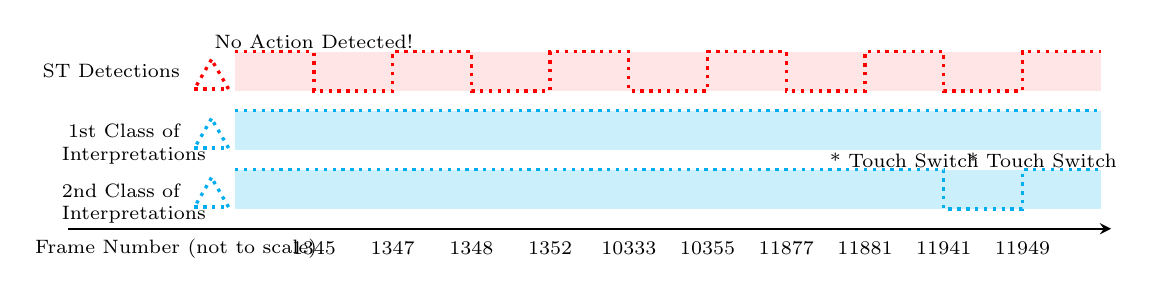
\begin{tikzpicture}[scale=0.5,>=stealth]
\scriptsize
\draw [thick,->] (-4.25,-0.5) -- (22.25,-0.5);
\node at (-1.5,-1) [] {Frame Number (not to scale)};
\node at (2,-1) [] {1345};
\node at (4,-1) [] {1347};
\node at (6,-1) [] {1348};
\node at (8,-1) [] {1352};
\node at (10,-1) [] {10333};
\node at (12,-1) [] {10355};
\node at (14,-1) [] {11877};
\node at (16,-1) [] {11881};
\node at (18,-1) [] {11941};
\node at (20,-1) [] {11949};
\fill [cyan!20] (0,0) rectangle (22,1);
\fill [cyan!20] (0,1.5) rectangle (22,2.5);
\fill [red!10] (0,3) rectangle (22,4);
\drawHiddenFluent{-0.6}{0.3}{0.5};
\drawHiddenFluent{-0.6}{1.8}{0.5};
\drawHiddenFluentST{-0.6}{3.3}{0.5};
\node at (-1,3.5) [label=left:ST Detections] {};
\node at (-1,2) [label=left:{\parbox{1.5cm}{\flushright 1st Class of\\Interpretations}}] {};
\node at (-1,0.5) [label=left:{\parbox{1.5cm}{\flushright 2nd Class of\\Interpretations}}] {};
\draw [very thick,red,dotted] (0,4) -- (2,4) -- (2,3) -- (4,3) -- (4,4) -- (6,4) -- (6,3) -- (8,3) -- (8,4) -- (10,4) -- (10,3) -- (12,3) -- (12,4) -- (14,4) -- (14,3) -- (16,3) -- (16,4) -- (18,4) -- (18,3) -- (20,3) -- (20,4) -- (22,4);
\draw [very thick,cyan,dotted] (0,2.5) -- (22,2.5);
\draw [very thick,cyan,dotted] (0,1) -- (18,1) -- (18,0) -- (20,0) -- (20,1) -- (22,1);
\node at (2,4.25) [] {No Action Detected!};
\node at (17,1.25) [] {* Touch Switch};
\node at (20.5,1.25) [] {* Touch Switch};
\end{tikzpicture}
%\includegraphics[trim = 0in 0in 0in 5.5in, clip, width=.98\linewidth]{lightdetections.pdf}
\caption{Given an ST detection that moves the light fluent between ON and OFF without a causing action, the reasoning process prefers this to be explained by incorrect detections of the light fluent.  The second most probable explanation is that two of the changes had causing actions that were missed by the detection.
 \label{fig:lightdetections}}
\end{figure*}


\subsection{Reference Estimates}

To evaluate performance on hidden and unobserved fluents, we compare the predicted fluent values by our algorithm with two types of reference estimates.

\begin{figure*}[htp]
\centering
\begin{tikzpicture}[scale=2.1,>=stealth]
\scriptsize
\node at (0,0) [label=below:485,label=left:{\bf$\cdots$}] {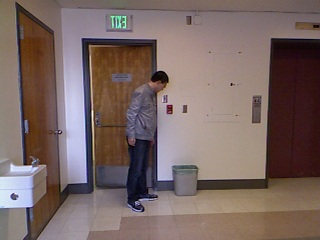
\includegraphics[width=.8in]{485}};
\node at (1,0) [label=below:800] {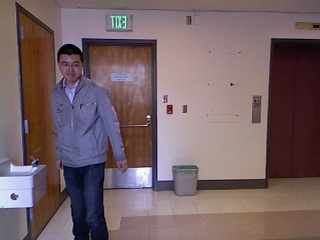
\includegraphics[width=.8in]{800}};
\node at (2,0) [label=below:2500] {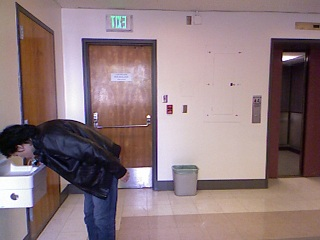
\includegraphics[width=.8in]{2500}};
\node at (3,0) [label=below:2575] {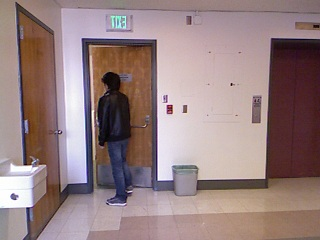
\includegraphics[width=.8in]{2575}};
\node at (4,0) [label=below:5535] {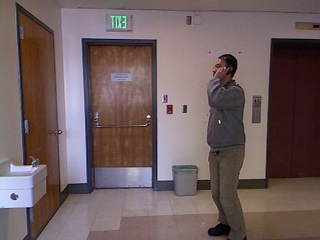
\includegraphics[width=.8in]{5535}};
\node at (5,0) [label=below:6915,label=right:{\bf$\cdots$}] {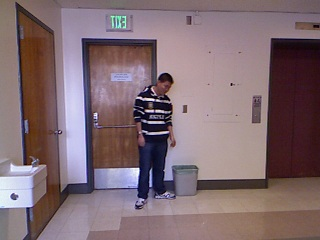
\includegraphics[width=.8in]{6915}};
\draw [->,thick] (-0.75,-0.6) -- (5.75,-0.6);
\node at (0,-0.6) [label=below:{Frame Number (not to scale)}] {};
\end{tikzpicture}
\caption{Sample of human judgment key frames. \label{fig:judgmentpoints}}
\end{figure*}

{\textbf{Human Estimates.}} A human experiment is performed through a website, allowing participants to complete the task at their own leisure. Each of 15 participating subjects is shown the test video which pause at preset frames, e.g., those shown in Figure~\ref{fig:judgmentpoints}. At each key frame, the subject is asked to assign a total of 100 points to all possible values of each fluent, according to his/her own (human) recognition and reasoning for events/actions and fluent changes. Assignment of the points correspond to the subjective probabilities of the fluent values, e.g., 90 points are assigned to COMPUTER ASLEEP if the subject feels it is 90\% likely that the computer is ASLEEP. The subject is allowed to revise previous judgments with information derived from subsequent frames. The recorded human judgments are taken as ground truth with a degree of variance, with which we can examine the performance of our algorithm against the distribution of human data.


{\textbf{Baseline Estimate.}} For a baseline estimate, the hidden fluents were assigned without using any detection or causal information. Their values are uniformly assigned, e.g., 50\% for LIGHT ON and 50\% for OFF. The baseline estimate is completely conservative without inclination to any observation or prior belief. The baseline estimate provides a discriminative reference against which we can see how well our algorithm approximates human performance. This reference point is very informative given the limited amount of human data (too limited to derive a reliable confidence interval with) whose true distribution is unknown.

TODO: use/include better baselines


\subsection{Experimental Results: inferring hidden fluents forward and backward in time}

Table~\ref{tab:comparison} shows numerically the performance of our algorithm in comparison to human and baseline. Values in the table are summarized based on $d(a,b)=\sum_{ij} d_{ij}(a,b)$, an accumulated distance between two estimates $a$ and $b$ over each fluent $i$ at key frame $j$, where $d_{ij}$ is the total variation (TV) distance between two assignments of the 100 points (equivalent to discrete probability distributions).

%\begin{table}[htp]
%\centering
%\caption{Comparison of computer, human and baseline estimates by TV distances. $c$, $b$ and $h$ represent computer, baseline and human estimates, respectively. $s$ and $t$ are indices for the collection of human estimates.\label{tab:comparison}}
%\begin{tabular}{c|cccc}
%\toprule
%& computer-baseline & computer-human & human-baseline & human-human \\
%& $d(c,b)$ & $\operatorname{mean}_s d(c,h_s)$ & $\operatorname{mean}_s d(h_s,b)$ & $\operatorname{mean}_{s\neq t} d(h_s,h_t)$ \\
%\midrule
%Hallway & 67.00000 & 37.50067 & 57.41622 & 33.46714 \\
%Office & 32.50000 & 58.67119 & 66.39667 & 31.26088 \\
%\bottomrule
%\end{tabular}
%\end{table}

\begin{table}[htp]
\centering
\caption{Comparison of computer, human and baseline estimates by TV distances. $c$, $b$ and $h$ represent computer, baseline and human estimates, respectively. $s$ and $t$ are indices for the collection of human estimates.\label{tab:comparison}}
\begin{tabular}{c|cc}
\toprule
 & Hallway & Office \\
\midrule
 computer-baseline, $d(c,b)$ &  67.00000 & 32.50000 \\
 computer-human,  $\operatorname{mean}_s d(c,h_s)$ & 37.50067 & 58.67119  \\
 human-baseline, $\operatorname{mean}_s d(h_s,b)$ & 57.41622 & 66.39667 \\
 human-human, $\operatorname{mean}_{s\neq t} d(h_s,h_t)$ & 33.46714 & 31.26088 \\
\bottomrule
\end{tabular}
\end{table}


\todo[inline]{include measures of how close the computer was to the human it was closest to.  }

\todo[inline]{maybe include distance computer was to median/mean human result}


For better visualization, these estimates (computer, human, and baseline) are reduced to two dimensions using multi-dimensional scaling (MDS) according to the TV distance between estimates, and plotted in Figure~\ref{fig:results}.

\begin{figure}[htp]
\centering
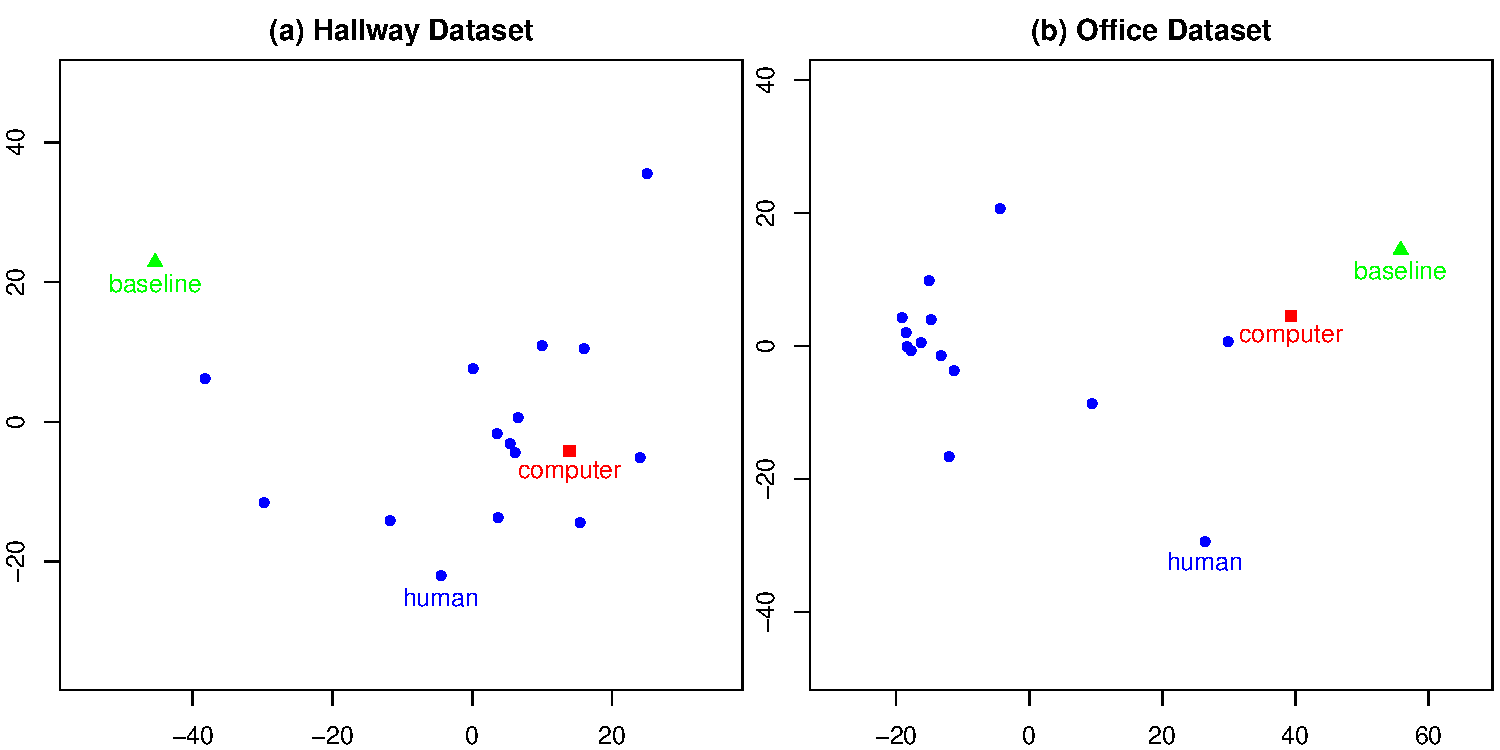
\includegraphics[trim = 0in 0in 5in 0in, clip,width=.75\linewidth]{results.pdf}
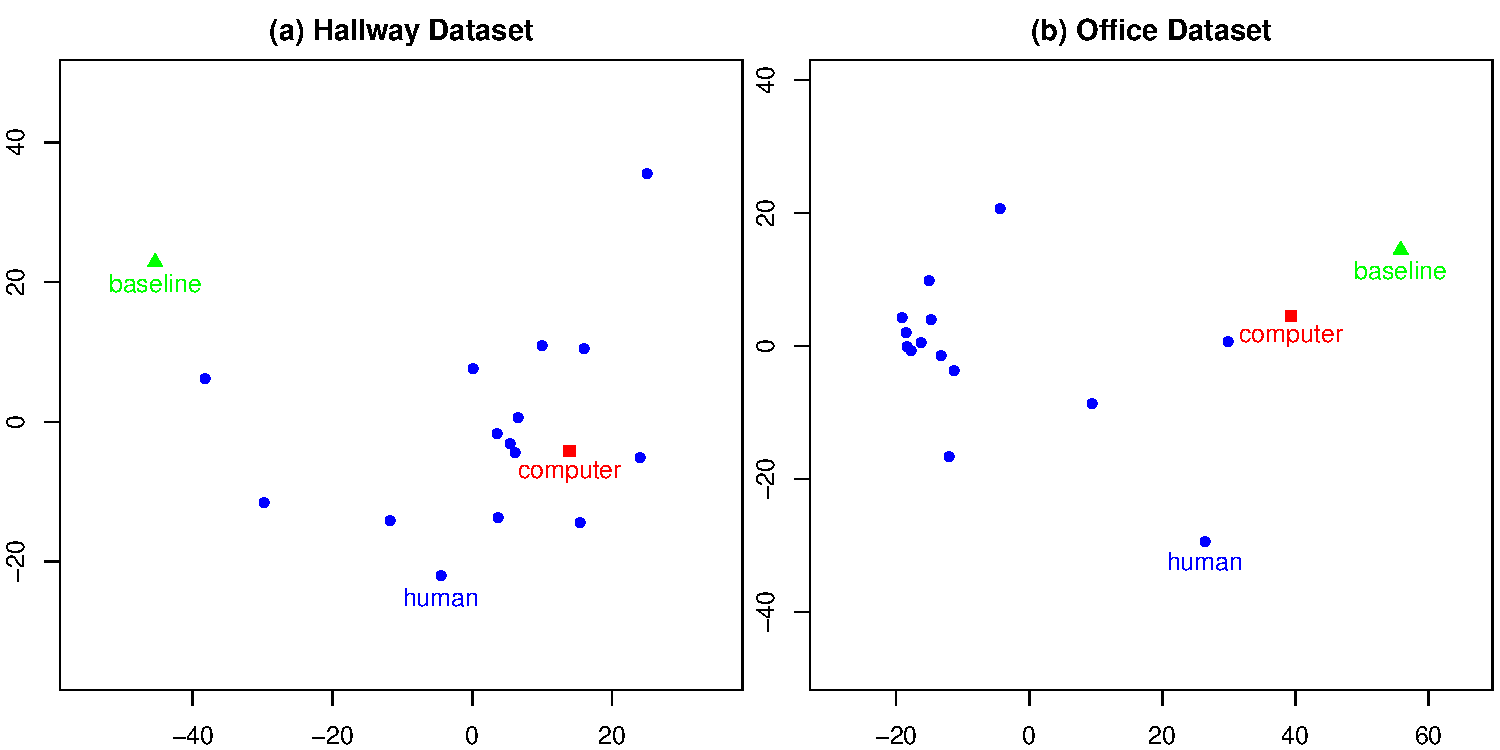
\includegraphics[trim = 5in 0in 0in 0in, clip,width=.75\linewidth]{results.pdf}
\caption{X-Y scatter plots of the 2D-embedded fluent value estimates using MDS. Red squares: estimates using our algorithm. Blue dots: human estimates. Green triangles: baseline estimates. \label{fig:results}}
\end{figure}

The hallway dataset contains observable fluent detections as well as actions. Both contribute to the causal inference of hidden fluents. The computer performance is very similar to human performance according to both the data and the plot. The baseline is away from the cluster of both.  The office dataset only contains detections of actions and all fluents are hidden and can only be inferred using the actions. The result is less satisfactory than that of the hallway data, but the computer performance still improves over the baseline towards human performance, as shown in Figure~\ref{fig:results}(b).






\subsection{Non-Markovian nature of data}

\todo[inline]{ show screensaver example, and show how markov process fails.}




\subsection{Joint parsing: causal and temoral information}

\todo[inline]{incorporate with the misinformation section/link more strongly, but point out difference.  corrections vs filling in missing information.}

TODO: show a few of instances:  1) light in hallway where we have temporal parsing...  using causal parsing improves results to ones in-line with humans. showcases C to T  2) light in office.  no spatial detection of light, so causal parsing completely dependent on (poor) detection of action. cautions about poor T.  3) a completely indetectable fluent, such as cup level.  so with the caveat that detection of hidden fluents is potentially unreliable without good action detection, it is possible to infer the hidden.


\section{Analysis of Experiments}

TODO: explain that the humans were far from each other, allowing leniency for the computer as well.   For the MDS, humans were actually quite far from each other for some of the check points, which gave the computer leeway overall.  Even with this disparity, the baseline confirms our performance is more in line with human estimations.

TODO: pick and choose graphs to include

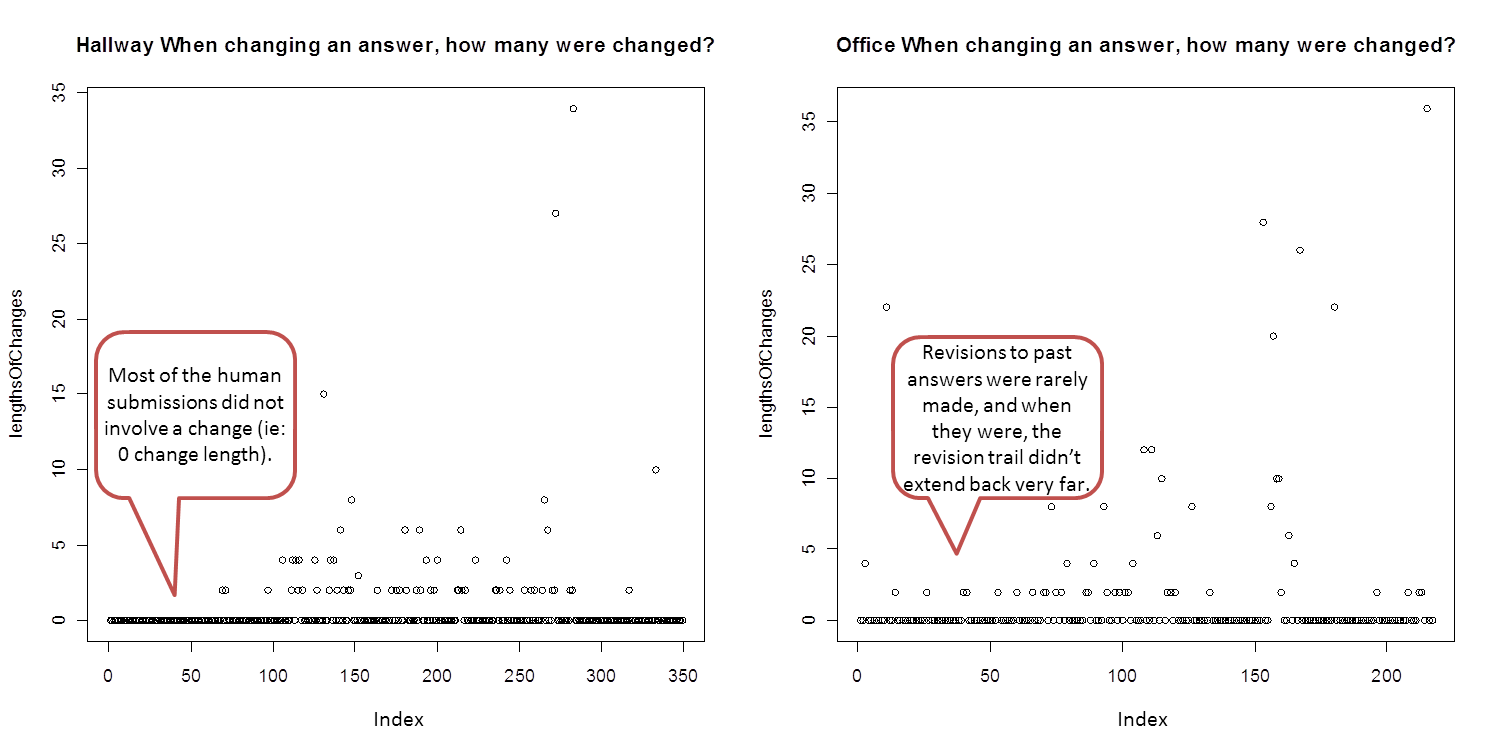
\includegraphics[width=0.9\linewidth]{Picture1.png}
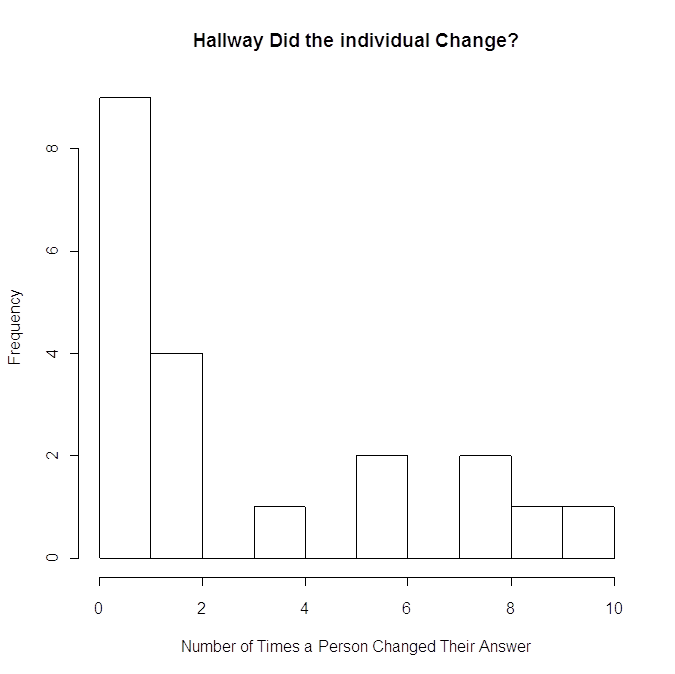
\includegraphics[width=0.4\linewidth]{Picture2.png}
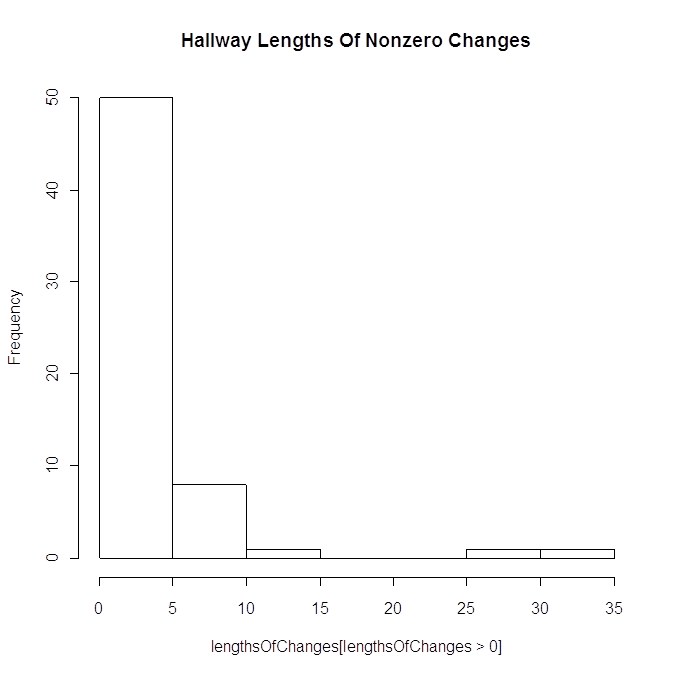
\includegraphics[width=0.4\linewidth]{Picture3.png}
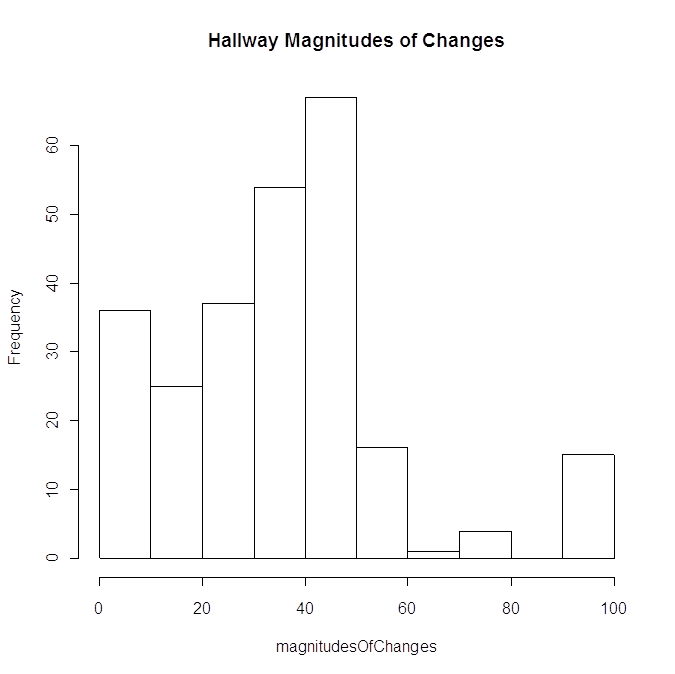
\includegraphics[width=0.4\linewidth]{Picture4.png}
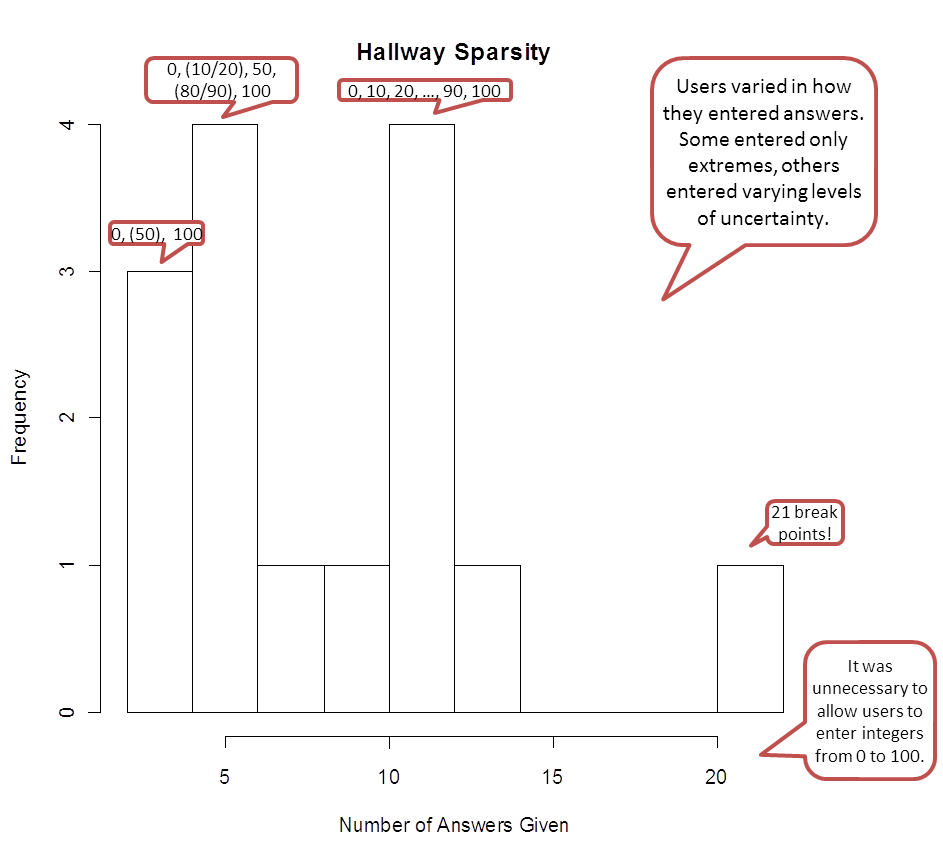
\includegraphics[width=0.4\linewidth]{Picture5.png}
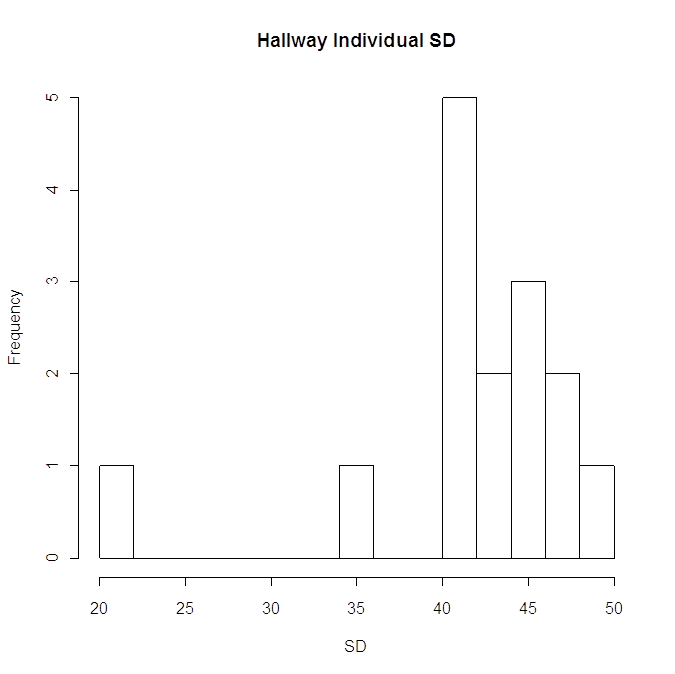
\includegraphics[width=0.4\linewidth]{Picture6.png}
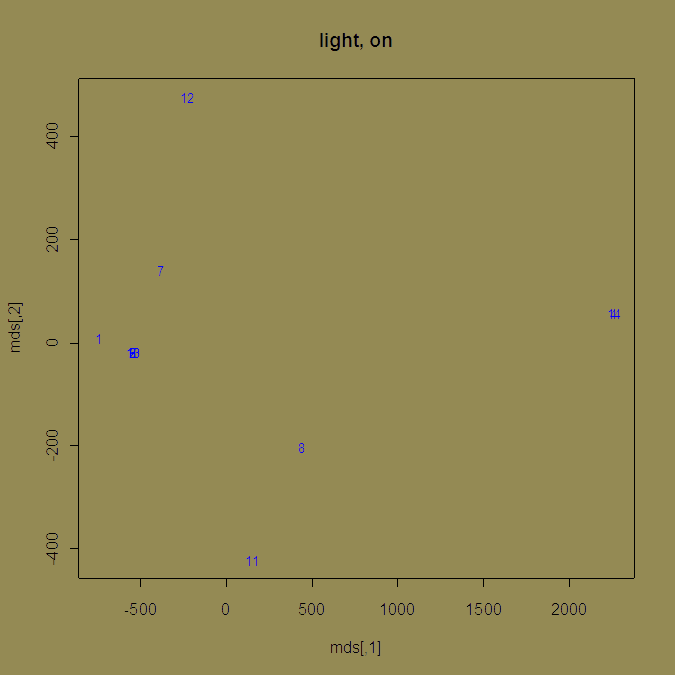
\includegraphics[width=0.4\linewidth]{Picture7.png}
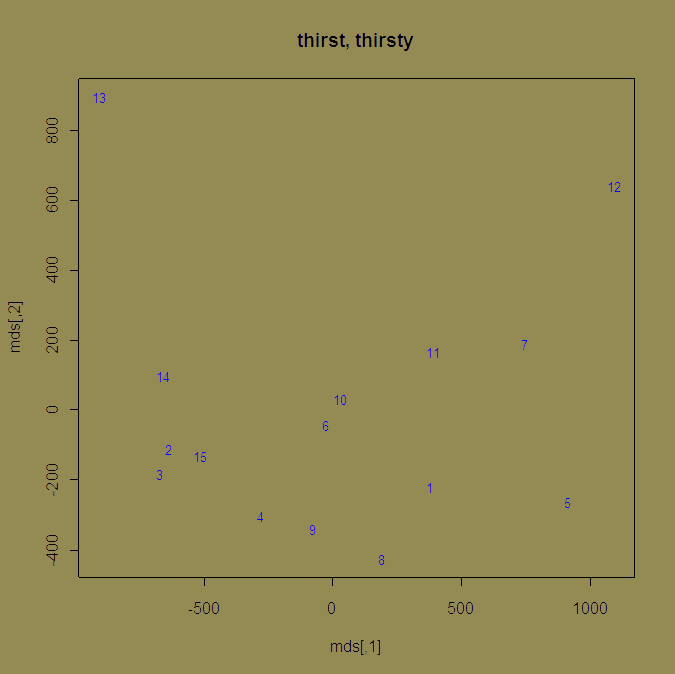
\includegraphics[width=0.4\linewidth]{Picture8.png}
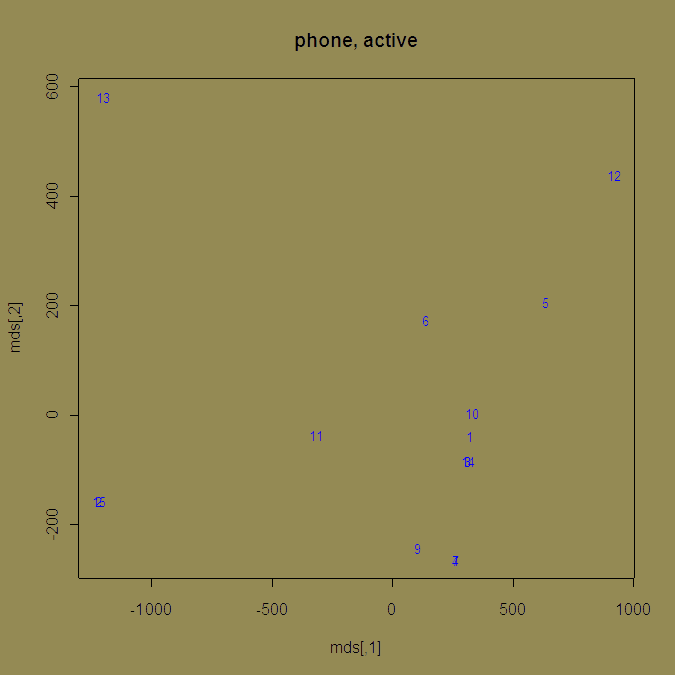
\includegraphics[width=0.4\linewidth]{Picture9.png}
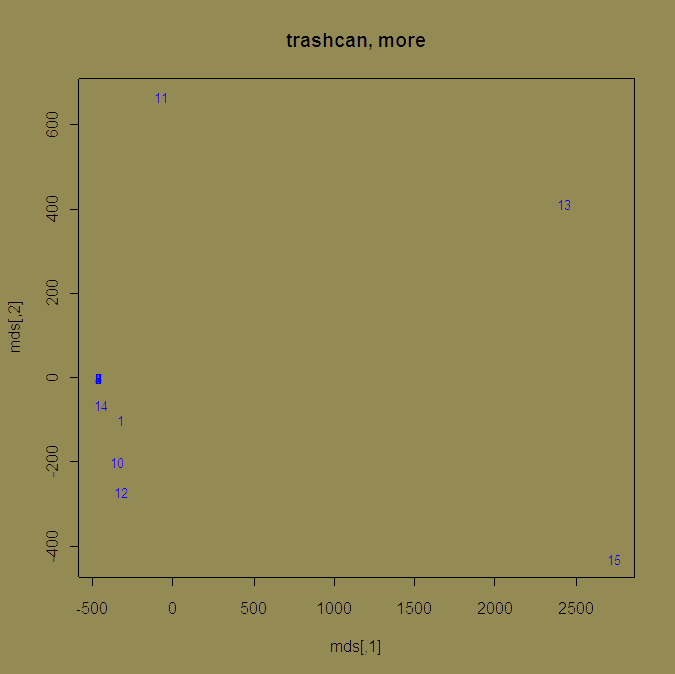
\includegraphics[width=0.4\linewidth]{Picture10.png}


\section{Discussion and summary of contributions}

This paper has introduced the dynamic C-AOG, which can infer the values of hidden fluents in video over a long duration, combining interpretations of multiple events backward and forward in time and binding these detections into a coherent sequence of explanations.

In addition to reasoning about top-level fluent consequences of actions, fluents were considered in terms of preconditions for an action to have an effect, in terms of internal trigger conditions (such as an agent's state of mind), and in terms of relative fluents where values were scalar rather than binary.

In experiments, inference was evaluated against baseline and human judgments.  The input to the system consisted of a single (incorrect by human judgment) ST description of the events.  For the hallway dataset, the system was presented with inconsistent information that it was able to reason through and find an explanation of the scene comparable to human judgments.  For the case of the office dataset, event detections were poor and no fluent detections were available to identify conflicts, leaving the system heavily dependent on those incorrect event detections.  Despite this disadvantage, the system was still able to use reasoning to outperform the baseline.

The results for the office dataset highlight the consequences of assuming too much from a single interpretation and reinforce the need to have multiple interpretations.  This paper presents some foundations for implementing the inference of hidden fluents.  Using this framework, joint inference of events and fluents can be used to  create a feedback system, allowing better detection of events.


%If a situation is unexplained by the C-AOG, all possible parse graphs will have low probability.  A current area of research is for the adaptive learning of the C-AOG.

%Want to reason about the hidden fluents, including the plan.  Want to go one step further: if plan not ideal, then want to guess what components he's missing.  (This is the discussion). 

%While this paper takes steps to predict hidden fluents, many more factors are incorporated as an agent plans his next move.  Much work is needed in order to fully anticipate an agent's plan of action.




% NEXT TIME: LIKE COUNTING CARDS IN VEGAS.  1) Computer better than human.  2) Doing it probabilistically helps determine future actions.

%COMPARISON TO NAIVE: WITH THINGS SUCH AS AGENT THIRST/SCREEN SAVER, WHERE THERE IS NO OBSERVABLE (OR UNDERSTOOD) CHANGE TO THIRSTY/DISPLAY OFF, THE NAIVE APPROACH EPIC FAILS.  TRIES TO RESOLVE EVERYTHING AS INERTIAL.  AND WHEN IT DOES PUT IN A CHANGE, IT'S UNSURE OF WHERE TO DO IT.

%NEXT TIME: how does phone ringing work.  how does reasoning it rang work.  because didn't push buttons.  

%\textbf{Conservative}.  For a conservative estimate, the hidden fluents were assigned without using any causal information.  The hidden fluents were randomly assigned as only one of the values.

%\textbf{Naive approach}.  Comparisons are offered to the naive approach as well.  Where actions are available, hidden fluents are filled in based on 

% NEXT TIME (maybe): \textbf{Markov approach}.
%*** : make sure used :) OOOH: term: "commonsense causality"  cool way to describe that we are not doing experiment design.

%Further, this naive approach relies quite heavily on the spatio-temporal detections, and will easily be confused in the presence of incorrect detections and conflict resolution thereof.  For example, if a person nears a light switch, but doesn't actually flip it, the ST detections will show the action happened, but the causal action did not.  

%NEXT TIME: maybe move that incorrect detection part elsewhere...  the caog fragment should handle it.  it's the hidden timeouts that are the real problem.

%Therefore, we need to probabilistically represent how long a fluent maintains status, in particular, how long the status stays in the inertial explanation.  

%\newpage
%
%\small
%\bibliographystyle{unsrt}
%\bibliography{../references/myrefs}
%\normalsize





% An example of a floating figure using the graphicx package.
% Note that \label must occur AFTER (or within) \caption.
% For figures, \caption should occur after the \includegraphics.
% Note that IEEEtran v1.7 and later has special internal code that
% is designed to preserve the operation of \label within \caption
% even when the captionsoff option is in effect. However, because
% of issues like this, it may be the safest practice to put all your
% \label just after \caption rather than within \caption{}.
%
% Reminder: the "draftcls" or "draftclsnofoot", not "draft", class
% option should be used if it is desired that the figures are to be
% displayed while in draft mode.
%
%\begin{figure}[!t]
%\centering
%\includegraphics[width=2.5in]{myfigure}
% where an .eps filename suffix will be assumed under latex, 
% and a .pdf suffix will be assumed for pdflatex; or what has been declared
% via \DeclareGraphicsExtensions.
%\caption{Simulation Results}
%\label{fig_sim}
%\end{figure}

% Note that IEEE CS typically puts floats only at the top, even when this
% results in a large percentage of a column being occupied by floats.
% However, the Computer Society has been known to put floats at the bottom.


% An example of a double column floating figure using two subfigures.
% (The subfig.sty package must be loaded for this to work.)
% The subfigure \label commands are set within each subfloat command, the
% \label for the overall figure must come after \caption.
% \hfil must be used as a separator to get equal spacing.
% The subfigure.sty package works much the same way, except \subfigure is
% used instead of \subfloat.
%
%\begin{figure*}[!t]
%\centerline{\subfloat[Case I]\includegraphics[width=2.5in]{subfigcase1}%
%\label{fig_first_case}}
%\hfil
%\subfloat[Case II]{\includegraphics[width=2.5in]{subfigcase2}%
%\label{fig_second_case}}}
%\caption{Simulation results}
%\label{fig_sim}
%\end{figure*}
%
% Note that often IEEE CS papers with subfigures do not employ subfigure
% captions (using the optional argument to \subfloat), but instead will
% reference/describe all of them (a), (b), etc., within the main caption.


% An example of a floating table. Note that, for IEEE style tables, the 
% \caption command should come BEFORE the table. Table text will default to
% \footnotesize as IEEE normally uses this smaller font for tables.
% The \label must come after \caption as always.
%
%\begin{table}[!t]
%% increase table row spacing, adjust to taste
%\renewcommand{\arraystretch}{1.3}
% if using array.sty, it might be a good idea to tweak the value of
% \extrarowheight as needed to properly center the text within the cells
%\caption{An Example of a Table}
%\label{table_example}
%\centering
%% Some packages, such as MDW tools, offer better commands for making tables
%% than the plain LaTeX2e tabular which is used here.
%\begin{tabular}{|c||c|}
%\hline
%One & Two\\
%\hline
%Three & Four\\
%\hline
%\end{tabular}
%\end{table}


% Note that IEEE does not put floats in the very first column - or typically
% anywhere on the first page for that matter. Also, in-text middle ("here")
% positioning is not used. Most IEEE journals use top floats exclusively.
% However, Computer Society journals sometimes do use bottom floats - bear
% this in mind when choosing appropriate optional arguments for the
% figure/table environments.
% Note that, LaTeX2e, unlike IEEE journals, places footnotes above bottom
% floats. This can be corrected via the \fnbelowfloat command of the
% stfloats package.







% if have a single appendix:
%\appendix[Proof of the Zonklar Equations]
% or
%\appendix  % for no appendix heading
% do not use \section anymore after \appendix, only \section*
% is possibly needed

% use appendices with more than one appendix
% then use \section to start each appendix
% you must declare a \section before using any
% \subsection or using \label (\appendices by itself
% starts a section numbered zero.)
%


%\appendices
%\section{Proof of the First Zonklar Equation}
%Appendix one text goes here.
%
%% you can choose not to have a title for an appendix
%% if you want by leaving the argument blank
%\section{}
%Appendix two text goes here.


% use section* for acknowledgement
\ifCLASSOPTIONcompsoc
  % The Computer Society usually uses the plural form
  \section*{Acknowledgments}
\else
  % regular IEEE prefers the singular form
  \section*{Acknowledgment}
\fi


The authors would like to thank... TODO.  Don't forget Ping's work (low-level action detection with the Kinect).


% Can use something like this to put references on a page
% by themselves when using endfloat and the captionsoff option.
\ifCLASSOPTIONcaptionsoff
  \newpage
\fi



% trigger a \newpage just before the given reference
% number - used to balance the columns on the last page
% adjust value as needed - may need to be readjusted if
% the document is modified later
%\IEEEtriggeratref{8}
% The "triggered" command can be changed if desired:
%\IEEEtriggercmd{\enlargethispage{-5in}}

% references section

% can use a bibliography generated by BibTeX as a .bbl file
% BibTeX documentation can be easily obtained at:
% http://www.ctan.org/tex-archive/biblio/bibtex/contrib/doc/
% The IEEEtran BibTeX style support page is at:
% http://www.michaelshell.org/tex/ieeetran/bibtex/
%\bibliographystyle{IEEEtran}
% argument is your BibTeX string definitions and bibliography database(s)
%\bibliography{IEEEabrv,../bib/paper}
%
% <OR> manually copy in the resultant .bbl file
% set second argument of \begin to the number of references
% (used to reserve space for the reference number labels box)



%%%%%%%%%  REFERENCES %%%%%%%%%%%

\bibliographystyle{IEEEtran}
\bibliography{IEEEabrv,../references/myrefs}




%\bibitem{IEEEhowto:kopka}
%%This is an example of a book reference
%H. Kopka and P.W. Daly, \emph{A Guide to {\LaTeX}}, third ed. Harlow, U.K.: Addison-Wesley, 1999.


%This is an example of a Transactions article reference
%D.S. Coming and O.G. Staadt, "Velocity-Aligned Discrete Oriented Polytopes for Dynamic Collision Detection," IEEE Trans. Visualization and Computer Graphics, vol.�14,� no.�1,� pp. 1-12,� Jan/Feb� 2008, doi:10.1109/TVCG.2007.70405.

%This is an example of a article from a conference proceeding
%H. Goto, Y. Hasegawa, and M. Tanaka, "Efficient Scheduling Focusing on the Duality of MPL Representation," Proc. IEEE Symp. Computational Intelligence in Scheduling (SCIS '07), pp. 57-64, Apr. 2007, doi:10.1109/SCIS.2007.367670.

%This is an example of a PrePrint reference
%J.M.P. Martinez, R.B. Llavori, M.J.A. Cabo, and T.B. Pedersen, "Integrating Data Warehouses with Web Data: A Survey," IEEE Trans. Knowledge and Data Eng., preprint, 21 Dec. 2007, doi:10.1109/TKDE.2007.190746.

%Again, see the IEEEtrans_HOWTO.pdf for several more bibliographical examples. Also, more style examples
%can be seen at http://www.computer.org/author/style/transref.htm

% biography section
% 
% If you have an EPS/PDF photo (graphicx package needed) extra braces are
% needed around the contents of the optional argument to biography to prevent
% the LaTeX parser from getting confused when it sees the complicated
% \includegraphics command within an optional argument. (You could create
% your own custom macro containing the \includegraphics command to make things
% simpler here.)
%\begin{biography}[{\includegraphics[width=1in,height=1.25in,clip,keepaspectratio]{mshell}}]{Michael Shell}
% or if you just want to reserve a space for a photo:



% insert where needed to balance the two columns on the last page with
% biographies
%\newpage

% You can push biographies down or up by placing
% a \vfill before or after them. The appropriate
% use of \vfill depends on what kind of text is
% on the last page and whether or not the columns
% are being equalized.

%\vfill

% Can be used to pull up biographies so that the bottom of the last one
% is flush with the other column.
%\enlargethispage{-5in}



% that's all folks
\end{document}



